% vim: spelllang=fr

\documentclass[../main.tex]{subfiles}
\graphicspath{{\subfix{../Figures/Chap1/}}}
\begin{document}

\begin{itshape}
Ce premier chapitre introduit les cyclones tropicaux (TC), de la simple définition jusqu'à la formulation de la question scientifique présentée dans cette thèse, en introduisant tous les concepts intermédiaires nécessaires.
\end{itshape}

\minitoc
%------------------------------------------------------------------------------------------------------------------
\section{Introduction aux cyclones tropicaux}

\subsection{Qu'est-ce qu'un cyclone tropical}\label{sec:quest_ce_qu_un_cyclone}

Du grec \textit{κύκλος}, nom commun désignant un cercle, ou plus généralement toute chose circulaire ou ronde, le terme cyclone, dans un contexte
météorologique, fait référence au type de circulation atmosphérique dans lequel l'air se trouve en rotation atour d'un centre de basse pression. Sous cette
définition, le terme de cyclone désigne une grande quantité d'objets aux caractéristiques très diverses et prenant place à différentes échelles spatiales et
temporelles. Ainsi, à la méso-échelle, ou échelle moyenne, caractérisée par des distances entre \km{10} et \km{100}, on peut par exemple citer les mésocyclones,
vortex d'air ascendant et convergeant, mesurant généralement moins de \km{10} de diamètre et observés dans les systèmes météorologiques convectifs, comme
notamment les orages super-cellulaires. De l'autre côté du spectre, à l'échelle synoptique, c'est à dire à l'échelle traitant des distances de l'ordre du
millier de kilomètres et sur des temps caractéristiques de quelques jours, les plus grands objets météorologiques dépressionnaires pouvant être qualifiés de
cyclones sont sans nulle doute les vortex polaires ; de larges dépressions d'altitude situées près des pôles géographiques et dans lesquelles de l'air froid est
en rotation. Malgré ces différences apparentes, tous les cyclones possèdent néanmoins des caractéristiques communes. Ainsi, le centre du cyclone est toujours
l'endroit où la pression atmosphérique est la plus faible, et la circulation de l'air autour du centre est assurée à minima par l'équilibre entre la force
induite par le gradient de pression radial d'une part, et la somme de la force centrifuge ainsi que la force de Coriolis d'autre part --- équilibre qualifié de
cyclostrophique, ou équilibre du vent gradient. La force de Coriolis, force inertielle causée par la rotation de la Terre, est également la raison pour laquelle
les cyclones tournent dans le sens contraire des aiguilles d'une montre dans l'hémisphère nord, et inversement dans l'hémisphère sud.

Les cyclones tropicaux ---~que l'on abrègera ensuite par l'acronyme TC, selon l'appellation anglaise \textit{Tropical Cyclone}~--- sont donc des phénomènes
tourbillonnaires pouvant atteindre plusieurs centaines de kilomètres, les plaçant ainsi à la lisière entre la mésoéchelle et l'échelle synoptique. Ces objets
prennent naissance, comme leur nom l'indique, dans la ceinture tropicale, définie comme la zone située entre le Tropique du Cancer dans l'hémisphère nord et le
Tropique du Capricorne dans l'hémisphère sud, et parfois approximée par la bande de \ang{20}S à \ang{20}N. Les TC se caractérisent par des vents violents autour
du cœur, appelé œil ainsi que des précipitations pouvant être très intenses et organisées par bandes au sein de la spirale cyclonique, et ont également la
propriété de posséder un cœur chaud en haute troposphère, c'est à dire une anomalie positive de température par rapport à leur environnement, propriété qui les
distingue des cyclones extra-tropicaux.
%
\begin{figure}[t]
    \centering
    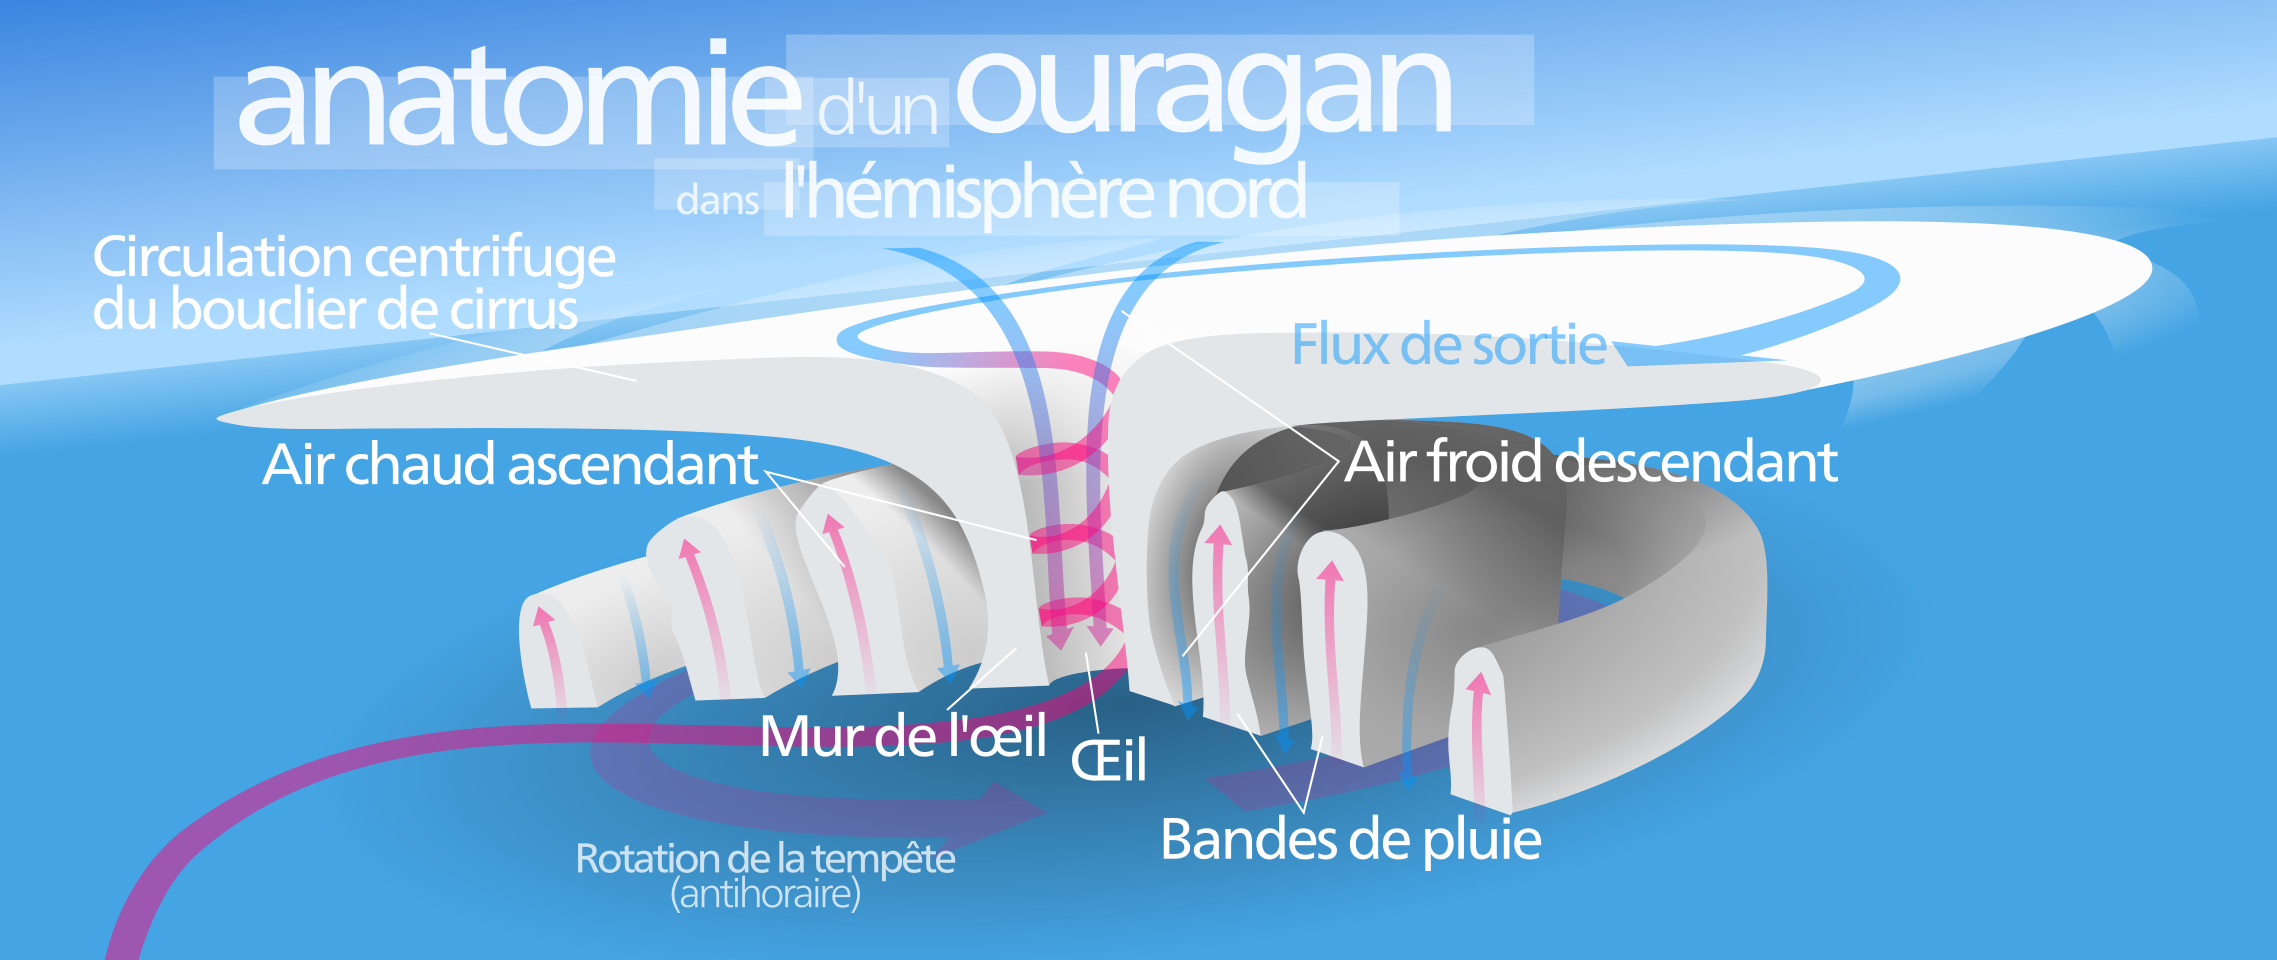
\includegraphics[width=0.9\textwidth]{Hurricane-fr.png}
    \caption{Diagramme en coupe d'un cyclone tropical, aussi appelé ouragan lorsqu'il survient dans l'océan Atlantique ou Nord-Est Pacifique --- By Kelvinsong -
    Own work, CC BY-SA 3.0, \url{https://commons.wikimedia.org/w/index.php?curid=23563610}}
    \label{fig:diagramme_TC}
\end{figure}
%
On dit que la perturbation dépressionnaire atteint le stade de cyclone tropical à proprement parler lorsque la vitesse du vent maximale à la surface et moyennée
sur une certaine période, variable selon les régions du monde, atteint le seuil de \ms{33}. En dessous de ce seuil, on parle soit de tempête tropicale si le
vent maximal est supérieur à \ms{17} ou bien de dépression tropicale si le vent maximal y est inférieur.

\subsection{Bassins d'activité et saisonnalité}\label{sec:bassins_saisons}

À l'échelle planétaire, il y a entre \numrange[range-phrase ={ et }]{82}{85} TC par an en moyenne selon les bases de données utilisées comme référence, et avec
un écart-type de \num{8} TC \parencite{schreck_impact_2014}. Cette activité globale est répartie sur un total de \num{6} grands bassins océaniques. Du point de
vue opérationnel, c'est à dire pour ce qui traite des aspects de surveillance et de prévision de l'activité cyclonique, ces bassins océaniques peuvent en
réalité être découpés en sous régions, dans lesquelles un centre météorologique régional spécialisé (CMRS, ou RSMC en anglais) ou un centre d'avertissements de
cyclones tropicaux (\textit{Tropical Cyclone Warning Centres}, TCWC) assure ces missions. Par exemple, l'océan Sud Indien est sous la tutelle conjointe, de part
et d'autre du 90\textsuperscript{ème} méridien Est, du CMRS de l'île de la Réunion (Météo-France) pour toute la partie Ouest, incluant le canal du Mozambique,
tandis que la surveillance de la partie Est est assurée par les TCWC de Perth, rattaché au Bureau of Meteorology (BoM) Australien, et de Jakarta. Néanmoins,
pour la régionalisation des analyses concernant l'activité cyclonique, nous favoriserons à travers ce document les grands bassins océaniques, et utiliserons des
définitions des domaines adaptées des recommandations de \cite{knutson_tropical_2020}, proposées dans un effort de standardisation afin de faciliter la
comparaison entre les études sur ce sujet. Ces bassins sont présentés sur la \cref{fig:bassins_TC}.
%
\begin{figure}[t]
    \centering
    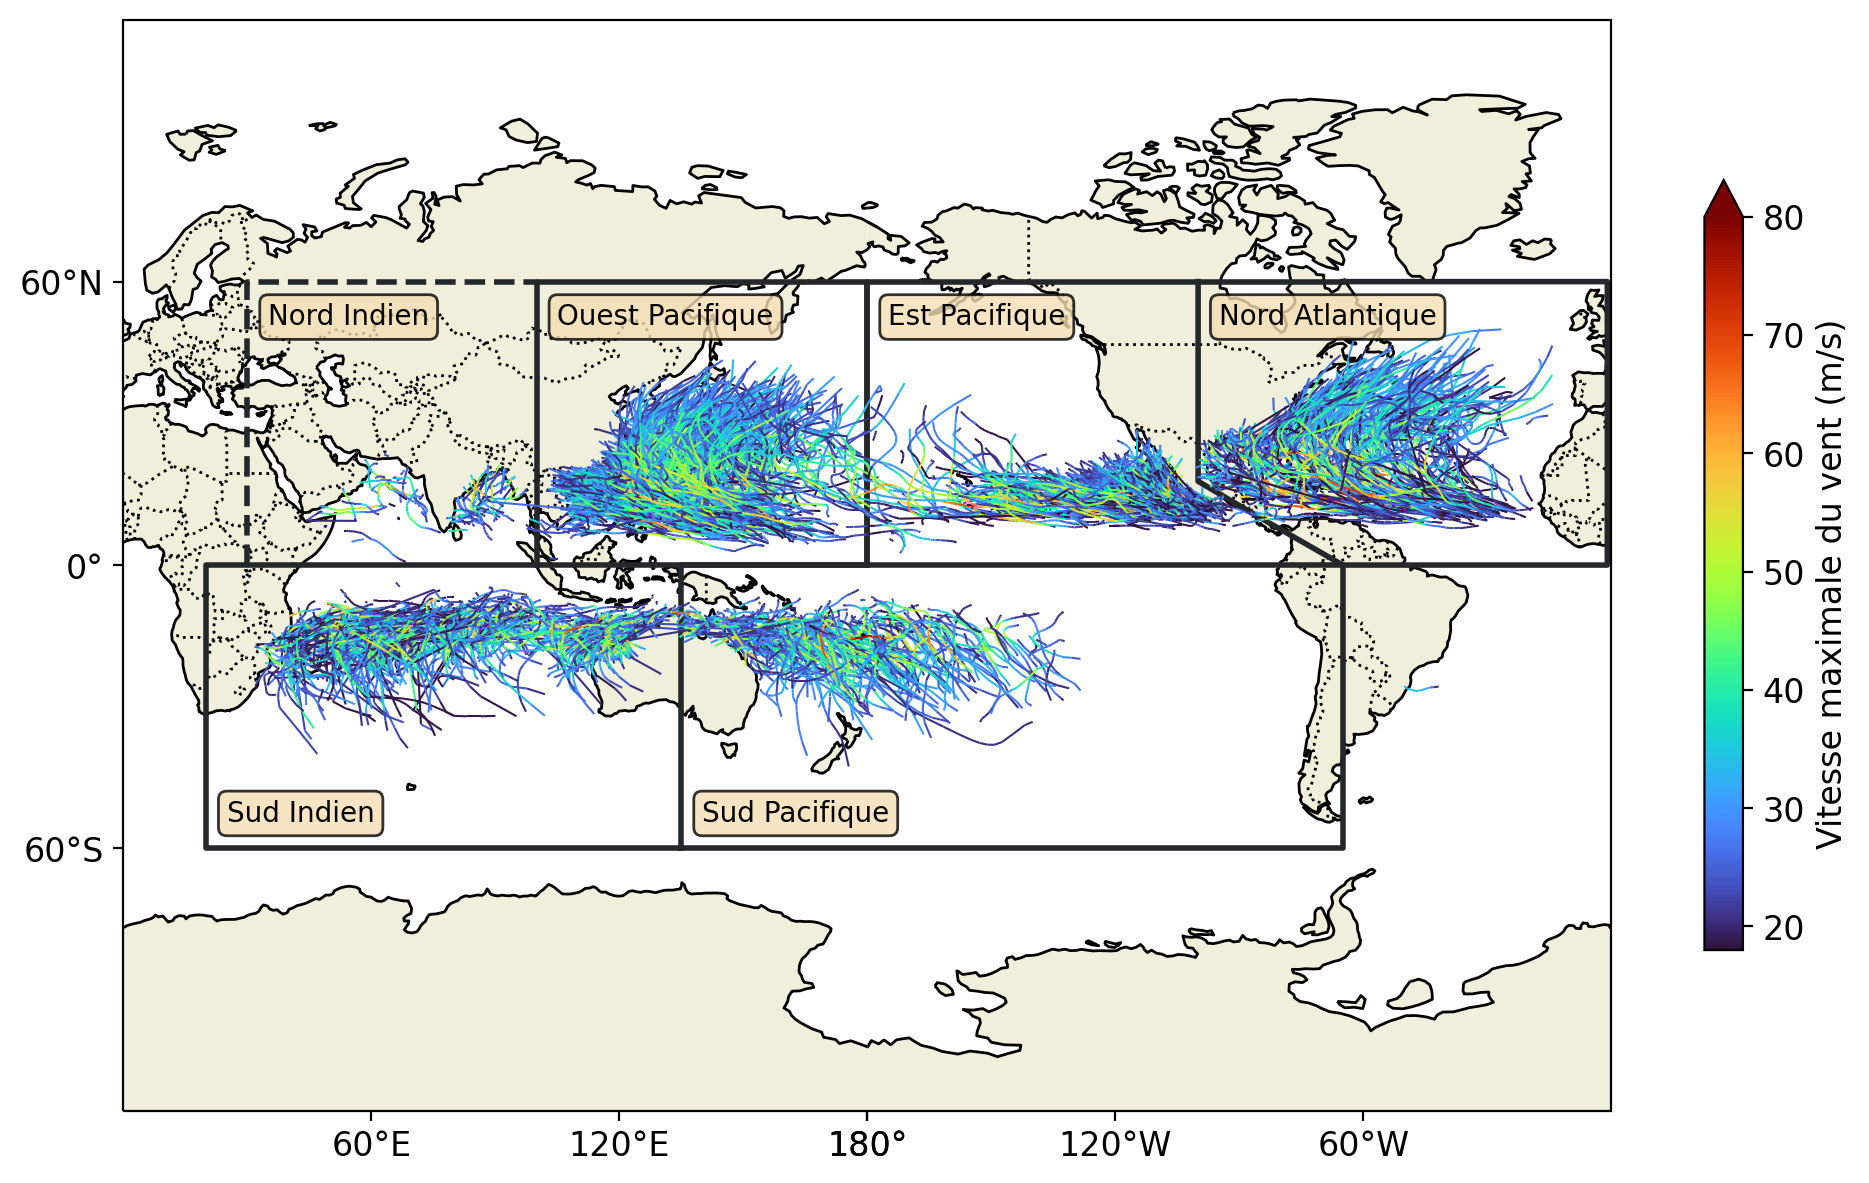
\includegraphics[width=0.9\textwidth]{Bassins_et_trajectoires.png}
    \caption{Bassins océaniques majeurs ainsi que les trajectoires des cyclones tropicaux observés entre 1981 et 2019, d'après la base de données
    \hbox{IBTrACS}. Les trajectoires sont colorées en fonction de l'intensité maximale des vents à chaque échéance. Les définitions des bassins océaniques
    utilisées ici, et plus généralement dans l'ensemble de ce document, sont issues, à quelques modifications près, des recommandations de \hbox{\cite[documents
    supplémentaires]{knutson_tropical_2020}}.}
    \label{fig:bassins_TC}
\end{figure}
%
Le bassin océanique concentrant la plus grande activité est le Ouest Pacifique (\textit{West Pacific}, WPac) avec environ \num{25} TC par an, ce qui représente
environ \SI{30}{\percent} de l'activité globale. Pour les autres régions de l'hémisphère nord ; en deuxième place se trouve le bassin Est Pacifique (EPac) avec
une moyenne de \num{16.5} TC par an, suivi du bassin Nord Atlantique (NAtl) avec \num{12} TC par an et enfin le bassin Nord Indien (NInd) avec entre \num{4} et
\num{5} TC par an, bassin le moins actif du monde \parencite{gray_global_1968,lander_look_1998,schreck_impact_2014}. Ce dernier se distingue également par le
fait que le pays possèdent en réalité deux zones d'activité, de part et d'autre des côtes Indiennes : sur la Mer d'Arabie, à l'Ouest, et dans la Baie du
Bengale, à l'Est. Au total, l'hémisphère nord contient \SI{70}{\percent} de l'activité cyclonique globale. En ce qui concerne l'hémisphère sud, ses \num{24} TC
annuels en moyenne sont répartis entre l'océan indien (\textit{South Indian}, SInd) et l'océan pacifique (\textit{South Pacific}, SPac) avec une moyenne de
\num{14.6} TC pour le premier et \num{9.4} TC pour le second. Il arrive parfois que des systèmes cycloniques se forment dans le sud de l'océan atlantique, bien
que la région ne soit pas considérée comme bassin cyclonique actif et qu'elle ne possède pas de CMRS. Le cas le plus notable, et l'unique système ayant atteint
le seuil de vent nécessaire pour être classé comme cyclone tropical, est le cas du cyclone Catarina, en mars 2004 et ayant frappé les côtés Brésiliennes alors
qu'il était au plus fort de son intensité \parencite{mctaggart-cowan_analysis_2006}. La portion de trajectoire correspondant à la partie la plus intense de ce
cyclone est d'ailleurs visible sur la \cref{fig:bassins_TC}.
%
\begin{figure}[t]
    \centering
    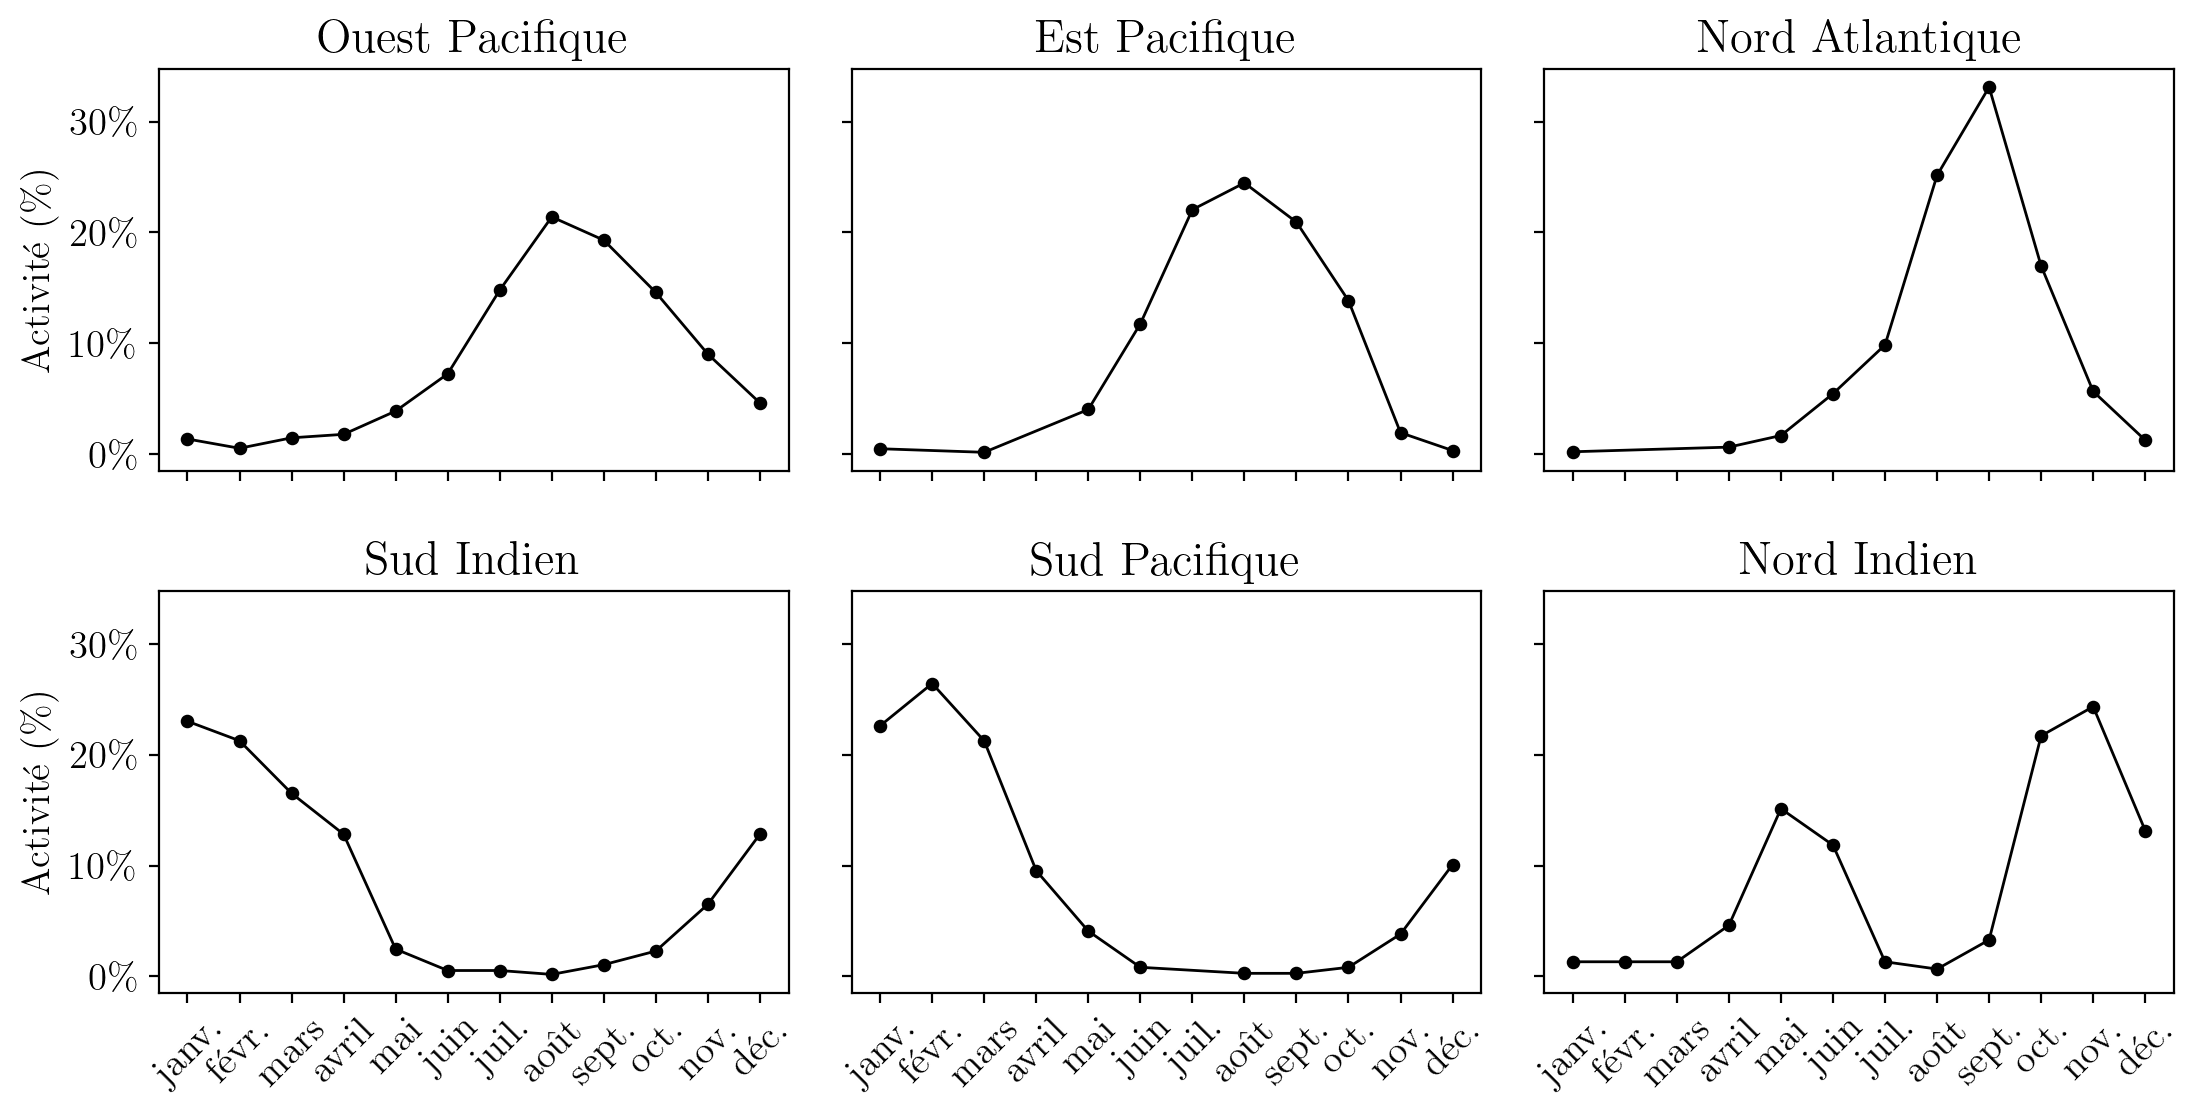
\includegraphics[width=\textwidth]{Saisons_TC.png}
    \caption{Saisonnalité de l'activité cyclonique tropicale dans les six bassins océaniques majeurs, normalisée pour chaque bassin et calculée à partir de la
    base de données IBTrACS entre 1981 et 2019 et en considérant pour chaque TC le mois de la première échéance où le stade de tempête tropicale est atteint.}
    \label{fig:saisons_TC}
\end{figure}
%
Les cyclones tropicaux surviennent principalement durant la saison chaude, avec plus ou moins d'étalement selon les régions, avec pour exception notable le cas
du bassin Nord Indien. Dans l'hémisphère sud, cela signifie que l'activité cyclonique est concentrée sur les mois de novembre à avril, avec la plus grande
partie située au delà de janvier, mais donc néanmoins répartie sur deux années calendaires. Pour cette raison, on considère dans l'hémisphère sud que les
saisons cycloniques courent de juillet de l'année précédente à juin de l'année courante, tandis qu'elle s'étend de janvier à décembre dans l'hémisphère nord. Le
cycle saisonnier des \num{6} bassins cycloniques majeurs est présenté sur la \cref{fig:saisons_TC}. Le bassin WPac présente la plus grande dispersion, avec une
activité comprise entre les mois de juin et de décembre, culminant au moins d'août. Pour l'EPac, la saison est un peu plus courte puisque, si elle commence
également autour de juin, le mois de novembre ne voit quant à lui quasiment aucune activité. Le bassin NAtl présente une activité encore plus recentrée avec un
pic en septembre qui concentre un tiers de l'activité du bassin. Le bassin SInd voit sa saison débuter en novembre avec un pic en janvier, tandis que le SPac
démarre un mois plus tard, en décembre, et présente un pic d'activité en février avec \SI{26}{\percent} de son activité qui est concentrée sur ce mois. Enfin,
le bassin NInd se distingue ici une fois de plus puisque son cycle annuel fait apparaître deux périodes d'activité. La première, mineure, prend place de avril à
juillet, tandis que la seconde, plus importante, a lieu de septembre à janvier. Cette coupure dans le cycle annuel s'explique par le phénomène de mousson
indienne, qui a lieu durant l'été, et qui apporte du cisaillement vertical dans l'atmosphère, élément défavorable à la cyclogénèse \parencite{gray_global_1968},
comme développé dans la \cref{sec:conditions_cyclogenese}.

\subsection{Risques associés et enjeux}

Les cyclones tropicaux constituent les événements météorologiques les plus extrêmes, les plus destructeurs et aussi les plus dangereux pour les populations.
D'après l'étude de \cite{doocy_human_2013}, le nombre médian de victimes par TC s'élève à \num{14} vies (\num{430} en moyenne), pour un bilan humain total
estimé entre les années 1980 et 2009 à \num{412644} morts et \num{290654} blessés. Les deux tiers de ce nombre sont attribués à seulement deux évènements : Le
cyclone Gorky de 1991 ayant fait \num{138866} victimes au Bangladesh, et le cyclone Nargis en 2008, en Birmanie, avec \num{138366} victimes. Outre les morts, le
nombre total de personnes affectées d'une façon ou d'une autre par les TC est estimé à plus de \num{466} millions, ce qui inclut \num{20} millions de personnes
qui se sont retrouvées sans abri. Ainsi, la région de l'Asie du Sud-est, telle que définie par l'Organisation Mondiale de la Santé, concentre \SI{80}{\percent}
des décès causés par les cyclones tropicaux, et \SI{53}{\percent} de la population affectée, tandis qu'elle ne concentre que \SI{9}{\percent} des évènements
impactants, ce qui montre alors que les plus forts impacts sont causés par quelques évènements extrêmes.

Pour ce qui est du coût des dégâts matériels associés aux TC, ils sont difficiles à estimer à l'échelle globale car ils n'ont étés rapportés que dans
\SI{15.4}{\percent} des cas, toujours d'après \cite{doocy_human_2013}. Ces coûts sont néanmoins d'autant plus importants que les pays concernés sont riches et
dotés d'infrastructures coûteuses. Le Centre National d'Information sur l'Environnement (NCEI) de l'Agence Américaine d'Observation Océanique et Atmosphérique
(NOAA) recense tous les évènements météorologiques extrêmes impactant les États-Unis dont les coûts dépassent le seuil de \num{1}~milliard de dollars. Ainsi,
entre 1980 et 2020, les dégâts causés par les cyclones tropicaux sont évalués, en tenant compte de l'inflation, à \num{1145.3}~milliards de dollars, ce qui
concentre \SI{52.3}{\percent} du coût total causé par l'ensemble des extrêmes météorologiques considérés ---~loin devant la deuxième plus importante cause de
dégâts matériels, à savoir les fortes tempêtes, qui concentrent \SI{15}{\percent} des coûts totaux~--- et ce qui représente un coût moyen de \num{21.6}~milliard
de dollars par évènement \parencite{smith_billiondollar_2020}.

Les risques associés aux TC sont nombreux et divers : vents extrêmes, fortes précipitations et inondations, orages, tornades et glissements de terrain. Mais le
plus grand risque provient des ondes de marées. Sous l'effet conjugué des vents et de la pression centrale du cyclone, le niveau de la mer augmente fortement et
rapidement, provoquant des inondations pouvant s'étendre sur plusieurs dizaines de kilomètres. Les ondes de marées sont le danger principal associé aux TC et
aussi la première cause de mortalité durant ces évènements \parencite{needham_review_2015}. Si chacun de ces risques peut, lorsque pris individuellement, causer
des pertes considérables, matérielles comme immatérielles, le danger est d'autant plus grand lorsque ces aléas surviennent simultanément et interagissent entre
eux, avec des impacts pouvant perdurer longtemps après le passage du cyclone. En effet, suite au passage d'un cyclone tropical, il n'est pas rare de voir
l'émergence de maladies infectieuses, en particulier dans les pays en voie de développement \parencite{shultz_epidemiology_2005}. Cette émergence se voit en
effet favorisée, entre autres, par la perturbation des infrastructures de santé publique ---~incluant les hôpitaux et les centres de soins, mais également les
réseaux de distribution en eau potable~--- mais aussi par les regroupements des populations dans des refuges surpeuplés, et plus généralement par une plus
grande exposition de ces derniers à l'environnement suite aux dommages causés aux habitations. Il en ressort donc que les dégâts matériels et économiques causés
par les cyclones tropicaux peuvent également avoir un coût en vies humaines.

Le plus un cyclone tropical est grand et développé, le plus les risques sont accrus. Bien qu'il soit difficile de déterminer précisément la relation liant d'une
part l'intensité d'un cyclone et les dégâts associés d'autre part, il est néanmoins admis que le potentiel de destruction d'un cyclone dépend au moins de
l'intensité de ses vents. Une métrique classiquement utilisée pour quantifier l'activité cyclonique sur une saison donnée consiste par exemple à faire la somme
des vents maximums soutenus, élevés au carré, avec une période de six heures, sur l'ensemble des systèmes de la saison lorsqu'ils dépassent au moins le stade de
tempête tropicale~--- métrique appelée l'énergie cumulative des cyclones tropicaux (\textit{Accumulated Cyclone Energy}, ACE, \cite{bell_climate_2000}). Si
d'autres métriques sont parfois utilisées et jugées plus pertinentes pour évaluer le potentiel destructeur d'un TC, elles restent toutefois basées sur la
vitesse du vent \parencite{powell_tropical_2007}. Ainsi, en supposant que le risque cyclonique demeure constant dans un climat plus chaud et que les pays
concernés par ce risque continuent à se développer, alors les dégâts économiques ne peuvent qu'augmenter. Sous cette hypothèse de stationnarité, les travaux de
\cite{ye_dependence_2020} suggèrent qu'un doublement de la valeur des actifs exposés à ce risque en Chine pourrait engendrer une hausse de \SI{80}{\percent} des
dégâts économiques induits par les TC. Or, rien ne permet d'affirmer la validité de cette hypothèse, étant données les incertitudes associées aux projections
futures de l'activité cyclonique tropicale (voir \cref{sec:projections_futures}). Par conséquent, l'évolution de l'activité cyclonique dans un contexte de
réchauffement global, en particulier pour ce qui concerne les questions d'intensité et de fréquence des TC, constitue un enjeu de première importance.

%----------------------------------------------------------------------------------------------------------------------
\section{Ingrédients de la cyclogénèse}
  
\subsection{Conditions de formation}\label{sec:conditions_cyclogenese}

On appelle \textquote{cyclogénèse} le processus par lequel un cyclone tropical se développe et s'intensifie. Bien que les mécanismes précis permettant
d'expliquer ce processus ne soient pas encore bien compris, malgré des décennies d'efforts consacrés à cette question \parencite{yanai_formation_1964,
montgomery_tropical_1993, gray_formation_1998, tory_tropical_2010}, il existe néanmoins un consensus quant aux facteurs qui y sont favorables. Les travaux de
\cite{gray_global_1968}, complétés dans \cite{gray_tropical_1975}, constituent, à partir des observations disponibles à l'époque, une étude globale sur
l'origine des cyclones tropicaux et font référence en la matière. Six facteurs sont ainsi identifiés et brièvement présentés ci-dessous.

\subsubsection{Vorticité relative en basses couches}

Les cyclones tropicaux se forment toujours à partir de perturbations atmosphériques préexistantes. Ce sont souvent des petits systèmes dépressionnaires
provenant de la zone de convergence intertropicale (ZCIT) \parencite{gray_global_1968}, ou encore des ondes d'est tropicales, comme dans le cas de l'océan
Atlantique où ces ondes peuvent jouent le rôle de précurseurs \parencite{thorncroft_african_2001,patricola_response_2018}. Ces perturbations apportent une
vorticité initiale, ou tourbillon, qui, par convergence frictionnelle, apporte de la vapeur d'eau provenant de la mer vers le cœur du système, au niveau de la
couche limite atmosphérique. Cette vapeur est entrainée en altitude par mouvement convectif, puis condensée, libérant de ce fait de la chaleur latente en haute
troposphère, contribuant ainsi à entretenir le fonctionnement du cyclone. Ce mécanisme constitue la source principale d'énergie des cyclones tropicaux
\parencite{emanuel_dependence_1987}.

\subsubsection{Rotation de la Terre}

La rotation de la Terre induit, du point de vue d'un observateur appartenant au même référentiel, une force sur tous les objets se déplaçant à la surface de la
planète et appelée force de Coriolis. Cette force, qualifiée d'inertielle ou de fictionnelle, en ce sens qu'elle n'est le résultat que du fait que le
référentiel d'observation est non inertiel, dévie les objets perpendiculairement à la direction de leur mouvement, vers la gauche si le référentiel tourne dans
le sens horaire et vers la droite si le référentiel possède une rotation anti-horaire. Dans le cas des cyclones tropicaux, la force de Coriolis tend à dévier
les cyclones vers les pôles géographiques (voir \cref{fig:bassins_TC}).

Mais outre l'effet sur leur trajectoires, la rotation de la Terre joue également un rôle primordial dans la circulation cyclonique, puisque c'est cette force
est à l'origine même du mouvement de rotation dans la circulation cyclonique. Cette force varie avec le sinus de la latitude et est donc nulle à l'équateur. À
proximité de l'équateur, la force de Coriolis est donc négligeable et les vents de la couche limite atmosphérique ne sauraient se maintenir au delà de quelques
mètres par secondes \parencite{gray_tropical_1975}. La force de Coriolis permet au vortex d'atteindre l'équilibre du vent gradient, mentionné dans la
\cref{sec:quest_ce_qu_un_cyclone} et donc de se développer jusqu'à devenir un cyclone tropical. Par conséquent, la cyclogénèse ne peut pas se produire à
l'équateur, et les observations historiques indiquent qu'une distance à l'équateur de \num{4}~à~\ang{5} est requise pour qu'un cyclone tropical puisse se
développer \parencite{gray_global_1968}.

\subsubsection{Faible cisaillement vertical du vent}

Le cisaillement du vent, ou plus précisément ici, le cisaillement vertical du vent horizontal, exprime la manière dont le vent horizontal varie avec l'altitude,
en intensité comme en direction. Dans le cas des cyclones tropicaux, on le mesure (ou le calcule) sur toute la hauteur de la troposphère, c'est à dire entre la
tropopause à \hPa{200} et la basse troposphère, typiquement à \hPa{850}. Le cisaillement détermine donc dans quelle mesure les couches supérieures de la
troposphère sont ventilées, ventilation qui limite donc la capacité du système à accumuler de la chaleur en son cœur \parencite{gray_tropical_1975}. Le
cisaillement vertical est donc très défavorable à la cyclogénèse.

\subsubsection{Température de surface de la mer}

Un cyclone tropical consomme environ \SI{15}{\mega\joule} par jour de chaleur sensible et latente extraite de la surface océanique
\parencite{gray_tropical_1975}. De plus, la circulation cyclonique produit une remontée d'eau océanique (upwelling) autour du centre du système. Pour ces
raisons, la cyclogénèse nécessite non seulement que la température de surface océanique (\textit{sea surface temperature}, SST) dépasse un certain seuil
---~évalué à \SI{26}{\degreeCelsius}, sinon quoi la flottabilité n'est pas suffisante pour assurer la convection \parencite{palmen_formation_1948}~--- mais
également que cette température soit atteinte sur au moins \m{60} de profondeur d'eau \parencite{leipper_observed_1967,perlboth_hurricane_1967}. En effet, si ce
seuil de SST n'est atteint qu'en surface, le phénomène d'upwelling apportera de l'eau plus froide qui ne permettra plus d'alimenter le système. Ce besoin
important en chaleur a généralement pour conséquence la désintensification rapide du TC mature lorsqu'il atteint les terres.

\subsubsection{Humidité relative et instabilité atmosphérique}

Ces deux derniers facteurs que sont l'humidité relative en moyenne troposphère, c'est à dire autour de \hPa{600}, et la notion de stabilité atmosphérique, sont,
dans le cadre de la cyclogénèse, étroitement liés. La stabilité de l'atmosphère, à fortiori lorsqu'elle est chargée en vapeur d'eau, dépend du gradient vertical
de température potentielle équivalente, notée $\theta_e$ et définie comme la température que la parcelle d'air atteindrait si tout son contenu en vapeur d'eau
venait à condenser et qu'elle était ramenée au niveau du sol de manière adiabatique. Le processus de convection des cumulonimbus, à l'origine de la formation
d'un cyclone tropical, nécessite en effet une forte diminution de $\theta_e$ entre la couche limite atmosphérique et la moyenne troposphère, c'est à dire une
atmosphère instable. Par ailleurs, la convection profonde est favorisée par une atmosphère à haute humidité relative en moyenne troposphère, car à température
égale, une parcelle d'air humide possède une plus grande flottabilité qu'une parcelle d'air sec. Enfin, toujours d'après \cite{gray_tropical_1975}, une humidité
relative élevée en haute troposphère favorise les précipitations et donc la libération d'enthalpie qui vient renforcer le cœur chaud du système.

\subsubsection{Climatologies}

La \cref{fig:clim_ingredients} présente les climatologies saisonnières de quatre des éléments favorables à la cyclogénèse que sont la vorticité absolue à
\hPa{850}, notée $\zeta_{\text{\hPa{850}}}$; l'humidité relative à \hPa{600}, $\text{RH}_{\text{\hPa{600}}}$ ; l'inverse du cisaillement vertical du vent
horizontal entre \hPa{200} et \hPa{850}, noté $1/S_z$ et enfin la SST relative aux tropiques. Ces champs sont issus de la réanalyse ERA5 du Centre européen pour
les prévisions météorologiques à moyen terme (CEPMMT, ou juste CEP ; en anglais \textit{European Centre for Medium-Range Weather Forecasts}, ECMWF)
\parencite{hersbach_era5_2020}, laquelle est décrite plus en détails dans la \cref{sec:chapitre_2}. Notons que la vorticité absolue $\zeta$ à \hPa{850} intègre
déjà le paramètre de Coriolis, noté $f$, auquel le module de la force éponyme est proportionnel, puisque la vorticité absolue est définie comme
\begin{equation*}
    \zeta = \zeta_R + \underbrace{2 \Omega \sin \phi}_{f}
\end{equation*}
\noindent où $\zeta_R$ est la vorticité relative, définie comme le rotationel du vent tel que mesuré dans le référentiel de la Terre, $\Omega$ la période de
rotation de la Terre et $\phi$ la latitude. L'inverse du cisaillement vertical est pris de telle façon à ce que des valeurs élevées indiquent des régions
favorables à la cyclogénèse et la SST est présentée ici comme la différence entre la SST et la température de surface moyenne entre \ang{20}S et \ang{20}N
---~nommée la SST relative~--- pour faire apparaître les variations saisonnières plus nettement.
%
\begin{figure}[tp]
    \centering
    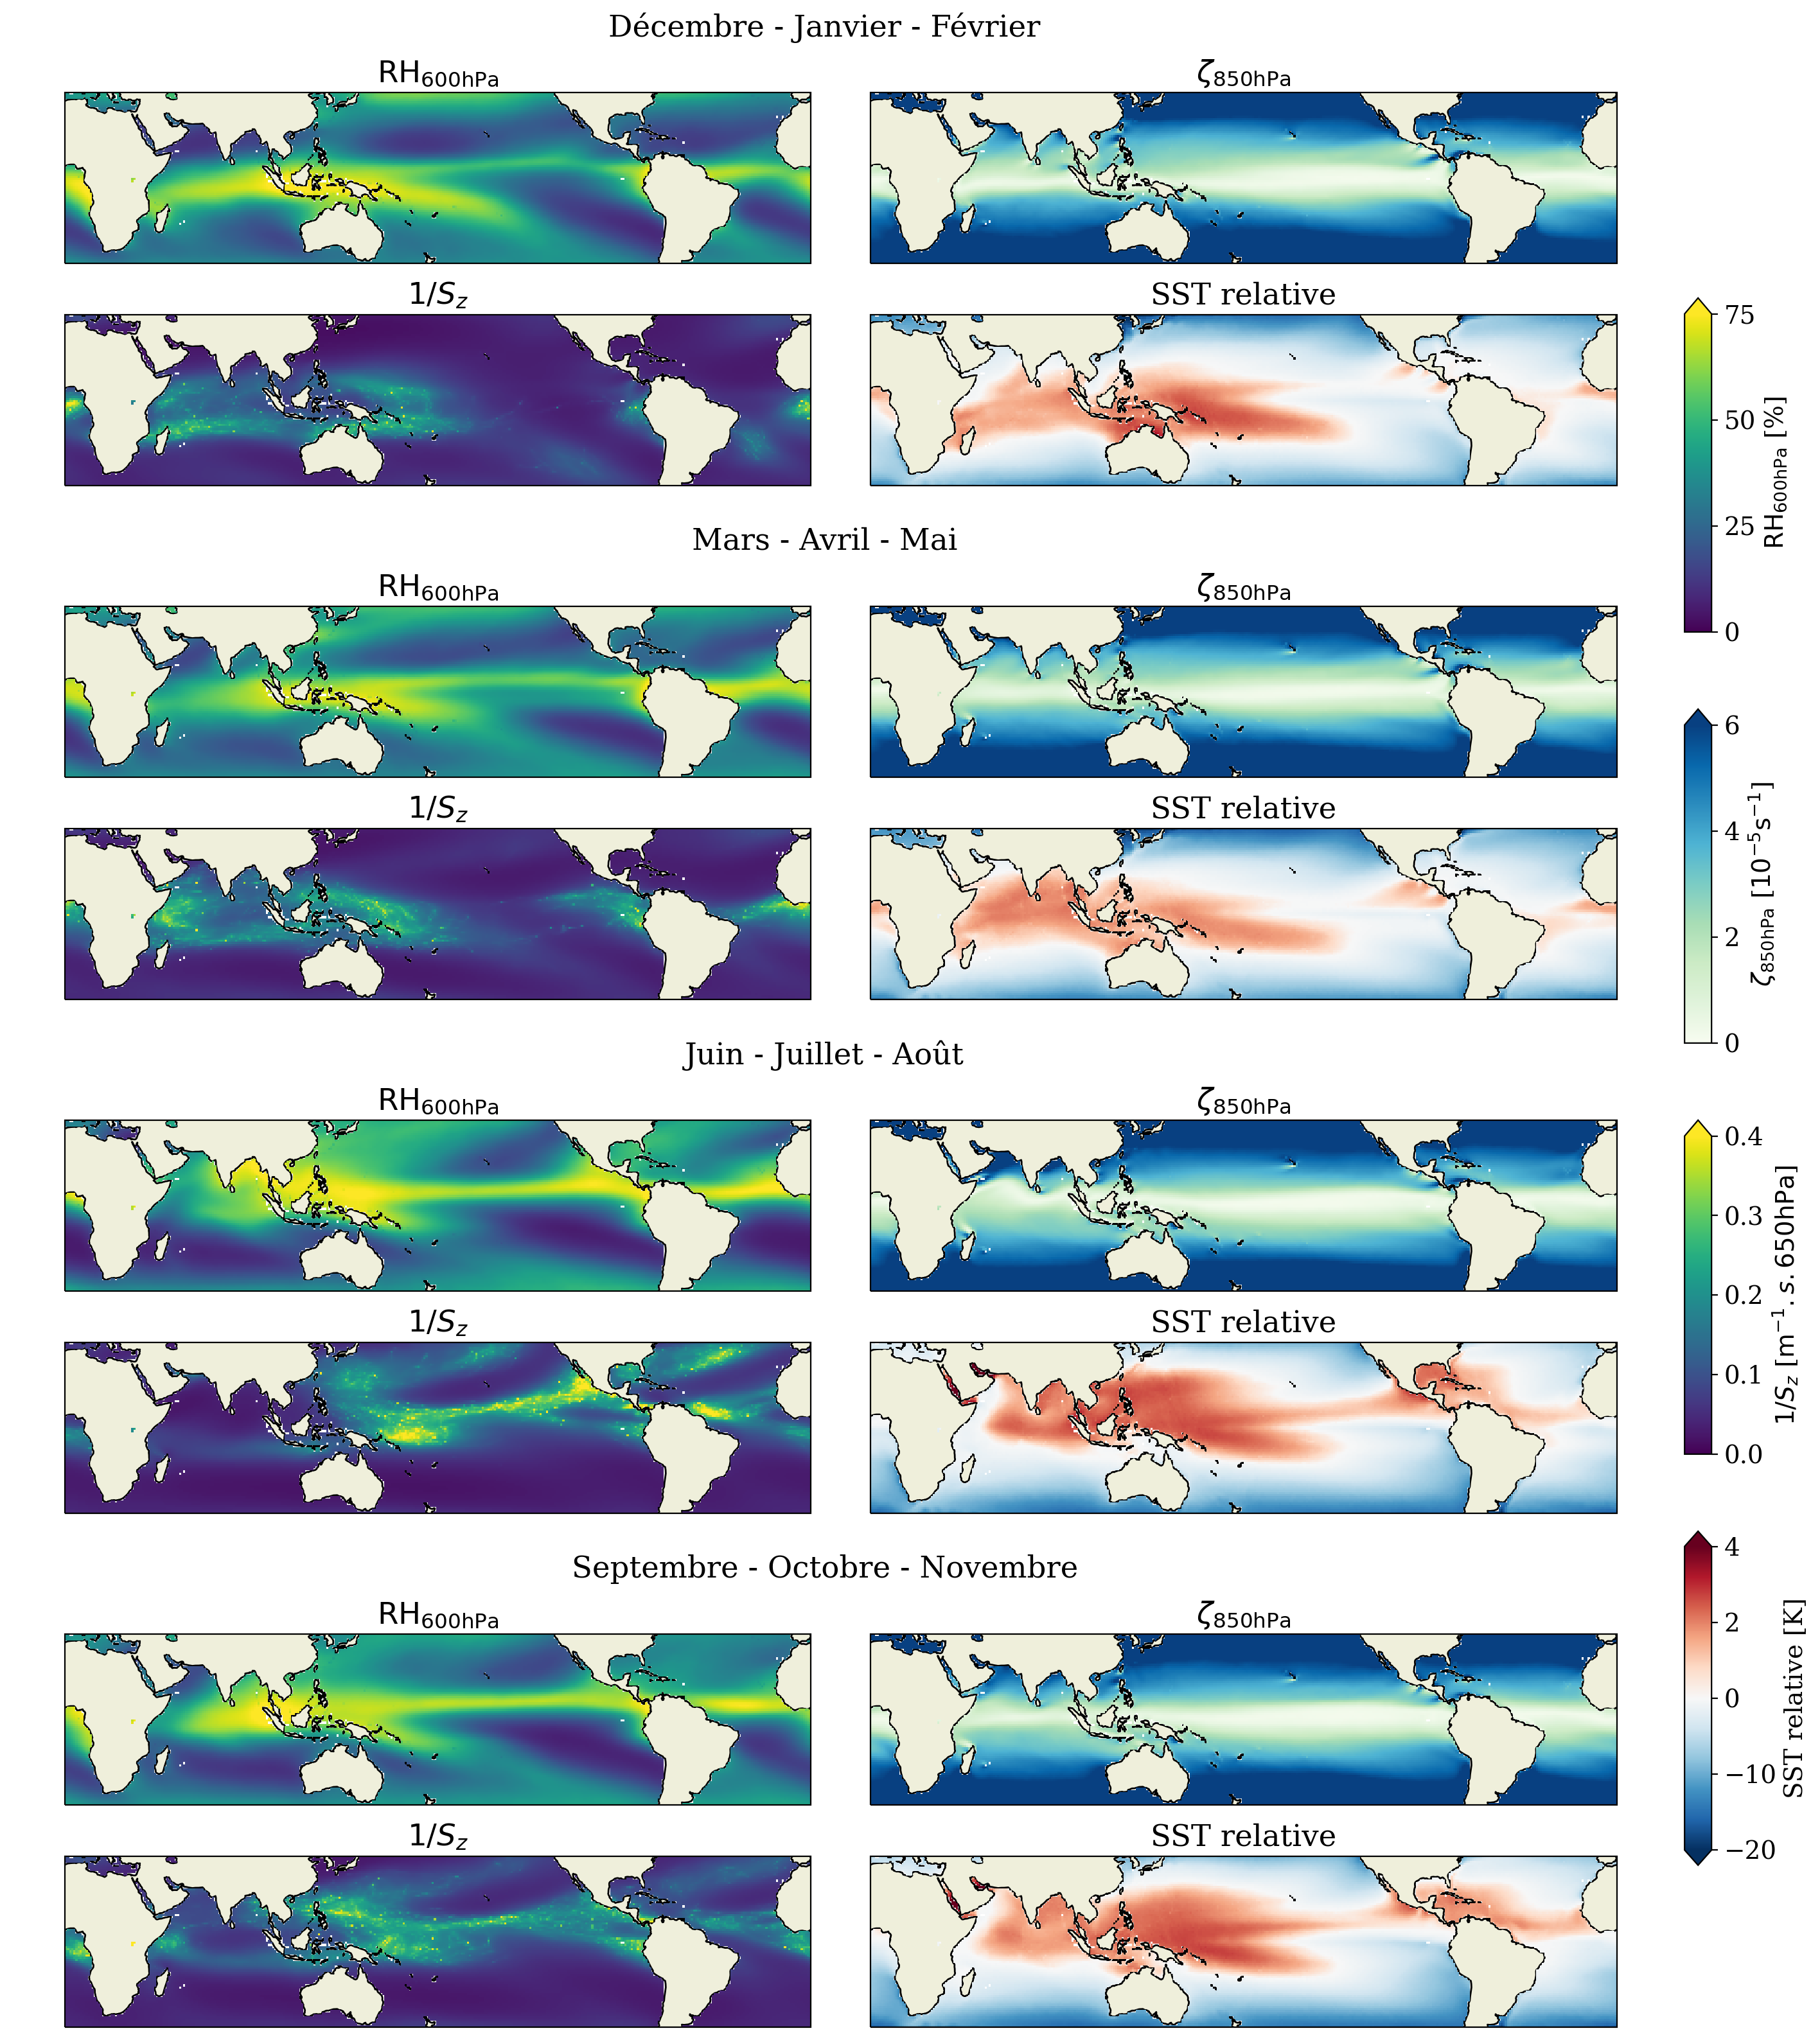
\includegraphics[width=\textwidth]{clim_saison_hurel_rotu_shear_sst.png}
    \caption{Climatologies saisonnières de l'humidité relative à \hPa{600}, de la vorticité absolue à \hPa{850}, de l'inverse du cisaillement vertical entre
    \hPa{200} et \hPa{850} et de la SST relative à la température moyenne le long de la ceinture tropicale, entre \ang{20}S et \ang{20}N, calculées à partir de
    moyennes mensuelles de la réanalyse ERA5 entre 1979 et 2020 et avec une résolution horizontale de \ang{1}.}
    \label{fig:clim_ingredients}
\end{figure}
%
Au premier abord, la SST apparaît comme un des facteurs prédominants dans la répartition spatiale et temporelle de l'activité cyclonique, puisqu'on retrouve sur
ces cartes de SST relatives la structure géographique des trajectoires de cyclones tropicaux observés présentés sur la \cref{fig:bassins_TC}. L'humidité
relative et le cisaillement laissent également apparaître cette répartition spatiale, avec toutefois quelques nuances supplémentaires, notamment dans les
régions extra tropicales. La climatologie de la vorticité est en revanche moins lisible mais présente localement des variations saisonnières dans l'étendue
méridionale du bandeau tropical. Par ailleurs, les variations saisonnières de ces quatre paramètres coïncident également avec l'activité mensuelle présentée sur
la \cref{fig:saisons_TC}. Cet accord est particulièrement visible sur les tracés de SST, avec des températures relatives de surface des océans très prononcées
dans l'Atlantique nord et l'Indo-Pacifique nord pendant les saisons Juin~-~Juillet~-~Août (JJA) ainsi que, dans une mesure un peu moindre, durant la saison
Septembre~-~Octobre~-~Novembre (SON). Cette configuration spatiale s'inverse dans l'Indo-Pacifique durant les saisons Décembre~-~Janvier~-~Février (DJF) et
Mars~-~Avril~-~Mai (MAM), où la partie sud présente une anomalie spatiale plus forte. Le bassin NInd durant la saison JJA constitue un cas particulier, déjà
évoqué précédemment (c.f \cref{sec:bassins_saisons}), puisque l'humidité relative, la vorticité et la SST y sont toutes trois élevées, tandis que l'activité
cyclonique y est quasi nulle (c.f \cref{fig:saisons_TC}). En effet, cette saison correspond à la mousson d'été en Inde, laquelle apporte du fort cisaillement
vertical, si bien que $1/S_z$ avoisine zéro. Cela illustre donc d'une part à nouveau le rôle essentiel du cisaillement dans le processus de cyclogénèse, et
d'autre part le fait que la cyclogénèse soit sensible à la combinaison de ces ingrédients.
%\noindent La climatologie de ces ingrédients fournit par ailleurs des indices sur la rareté des cyclones tropicaux dans l'océan Atlantique sud. La SST ne
%s'éloigne guère de la moyenne tropicale tout au long de l'année, l'humidité y est beaucoup moins présente que dans les autres bassin d'activité et la région
%présente par ailleurs du cisaillement, avec une baisse durant DJF. Selon \cite{gray_global_1968}, il n'y a généralement pas de ZCIT dans ce secteur non plus,
%ce qui prive la région des précurseurs qui peuvent en être issus. 

En première approche, il est possible d'estimer la climatologie spatiale et saisonnière des zones où les conditions favorables sont réunies en prenant
simplement le produit des quatre variables présentées sur la \cref{fig:clim_ingredients}. C'est ce que montre la \cref{fig:produit_ingredients}, avec en
superposition les premières observations des trajectoires des cyclones tropicaux observés entre 1981 et 2019, celles là mêmes qui sont présentées sur la
\cref{fig:bassins_TC}. Ce produit est ici défini comme suit :
\begin{equation*}
    \text{RH}_{\hPa{600}} \times \zeta_{\hPa{850}} \times \frac{1}{S_z} \times \text{SST} \quad \text{[$10^{-5}$ K m$^{-1}$ \hPa{650}}]
\end{equation*}
\begin{figure}[tbp]
    \centering
    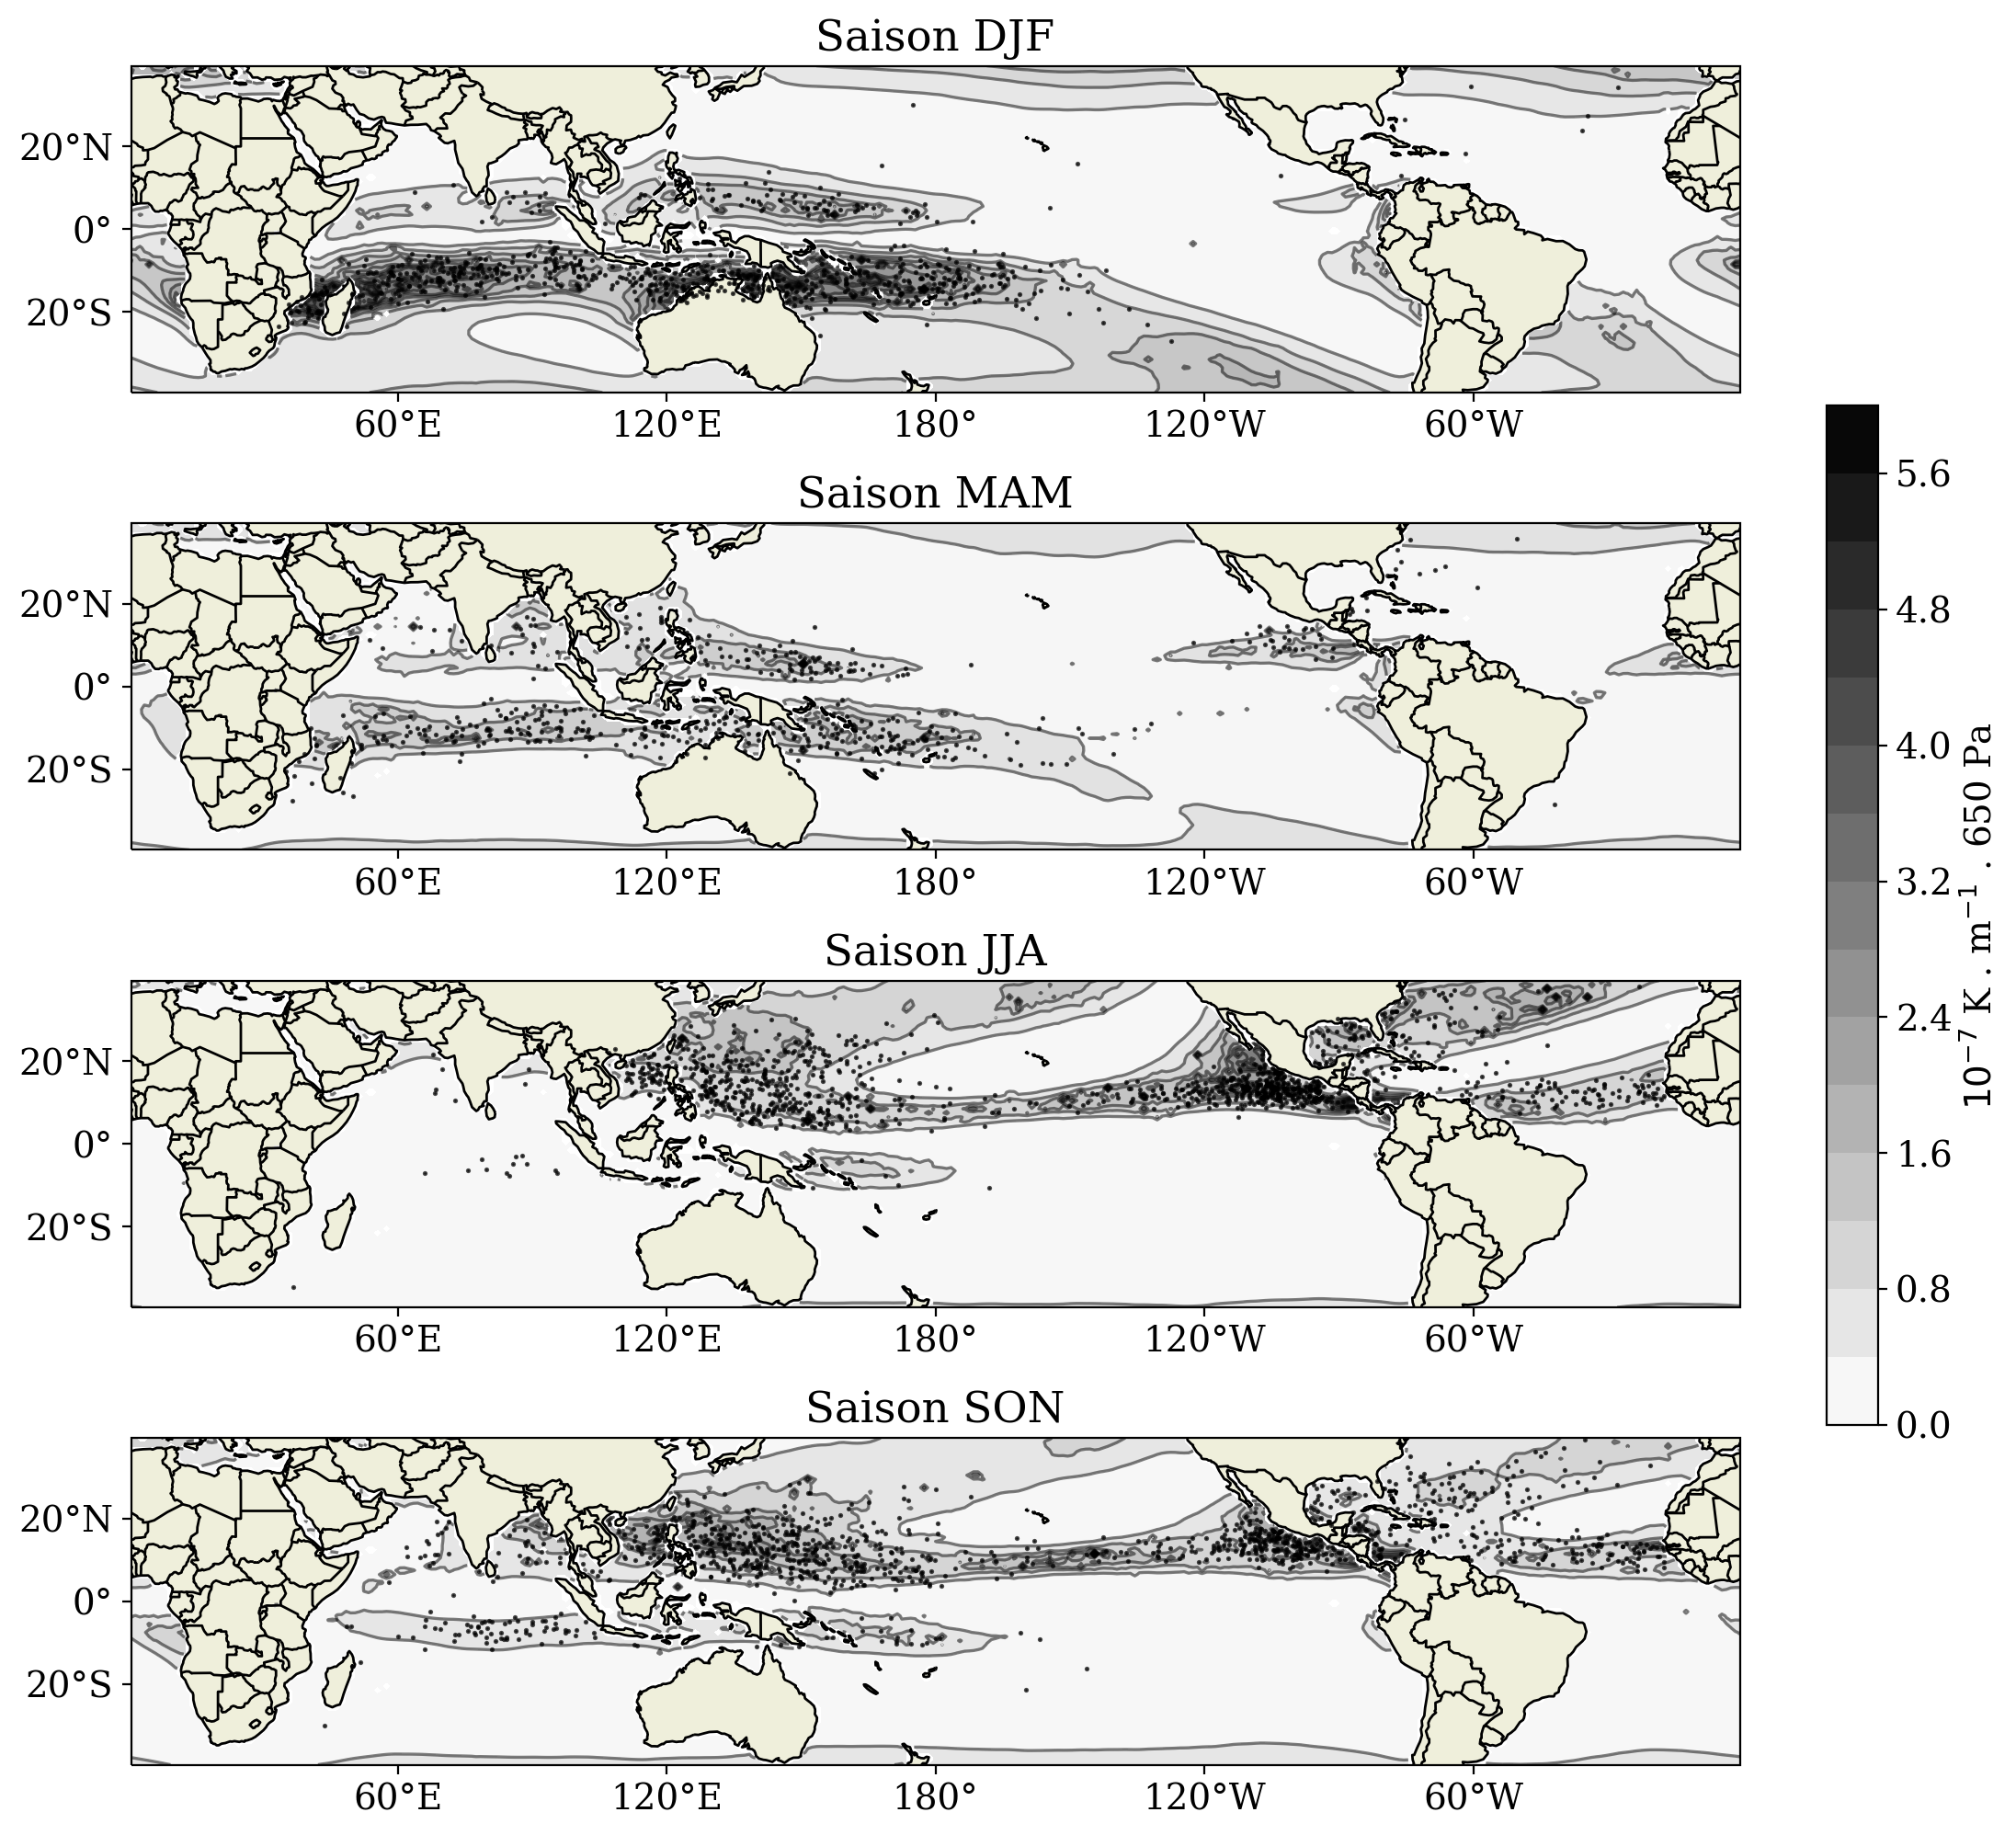
\includegraphics[width=1\textwidth]{clim_saison_produit_ingredients_et_ibtracs.png}
    \caption{Climatologies saisonnières du produit des quatre variables présentées sur la \cref{fig:clim_ingredients}, où la SST est ici simplement la
    température de surface de l'océan, sans considérer l'écart aux tropiques. Sont représentés par des points noirs pour chaque saison les premières
    observations des trajectoires présentées sur la \cref{fig:bassins_TC}.}
    \label{fig:produit_ingredients}
\end{figure}
\noindent Cette figure montre un excellent accord entre le produit des quatre variables et l'activité cyclonique observée, aussi bien dans la répartition
géographique que temporelle. Quelques points de discorde demeurent cependant, notamment durant les saisons DJF et SON dans l'océan Pacifique sud et nord,
respectivement, où la combinaison des variables indique des zones favorables jusque dans les moyennes latitudes, tandis que l'activité cyclonique y est quasi
inexistante. On distingue dans ces zones l'empreinte conjointe de l'humidité relative et du cisaillement, lesquelles présentent la même structure durant ces
saisons sur la \cref{fig:clim_ingredients}. Dans la ceinture tropicale et sub-tropicale, la correspondance entre le produit des paramètres et l'activité
observée demeure cependant remarquable. Ce constat selon lequel la fréquence d'occurrence des cyclones tropicaux en un lieu donné puisse être proportionnelle à
une combinaison de variables de grande échelle, découverte attribuée à \cite{gray_tropical_1975}, est à l'origine de ce qui sera nommé par la suite les indices
de cyclogénèse, et qui seront abordés plus en détails dans la \cref{sec:tracking_vs_indices}, puis dans le \cref{sec:chapitre_3}.

% \subsection{Modèles conceptuels de fonctionnement}
% 
% \subsubsection{CISK}
% 
% \cite{charney_growth_1964,ooyama_dynamical_1964,ooyama_numerical_1969}
% 
% \subsubsection{WISHE}
% 
% \cite{emanuel_airsea_1986,emanuel_largescale_1994}

%----------------------------------------------------------------------------------------------------------------------
\section{Cyclones tropicaux et changement climatique}

\subsection{Bases de données observationnelles et tendances historiques}

Un pré-requis pour pouvoir traiter de changement climatique, quelque soit l'objet d'étude, est de disposer de données observationnelles le plus fiables
possibles, et sur la plus longue période possible. Un des problèmes fondamentaux avec les réseaux d'observation météorologiques en général, est que les
instruments s'améliorent avec le temps, les réseaux s'étendent et se densifient, ce qui donne lieu à des fortes hétérogénéités et ruptures temporelles dans la
qualité des données. L'observation des cyclones tropicaux ne fait pas exception à cette règle. Les cyclones étant des phénomènes prenant place sur mer, les
premiers relevés météorologiques de cyclones tropicaux étaient réalisés par les marins et consignés dans leurs journaux de bords
\parencite{knapp_international_2010}. Avec le temps, et étant donné le fort potentiel d'impact de ces systèmes, les sources d'observations se sont multipliées
et diversifiées, de manière très inégale selon les régions. Les États-Unis déploient par exemple des avions de reconnaissances dédiés à la recherche et à
l'observation des cyclones tropicaux au large des côtes atlantiques depuis \num{1946}, bassin océanique qui est encore à ce jour le seul à bénéficier de ce type
d'observations de manière régulière. D'autres sources d'observations incluent notamment les stations météorologiques terrestres, bouées instrumentées, radars et
enfin radio sondages, ces derniers pouvant être réalisés par largage aérien directement dans le cyclone. Néanmoins, la véritable rupture technologique a lieu
avec l'ère satellitaire, réellement entérinée à la fin des années 70. L'observation par satellite permet d'une part de détecter la quasi totalité des cyclones,
mais aussi d'estimer systématiquement leur intensité, même en l'absence de mesures \textit{in situ}, par analyse de Dvorak consistant en une estimation
indirecte et partiellement subjective de l'intensité à partir de la structure des amas nuageux et de leur température
\parencite{dvorak_tropical_1975,velden_development_1998,olander_development_2002,olander_advanced_2007,olander_advanced_2019}\footnote{Le perfectionnement de la
méthode de Dvorak originelle avec le temps est indicatif du fait que les données observées relatives à l'intensité des cyclones tropicaux souffrent
d'hétérogénéité temporelle, et ce même après le début de l'ère satellitaire.}. En effet, un bon nombre de systèmes qui n'atteignaient jamais les côtes passaient
inaperçus avant cela \parencite{landsea_atlantic_2004}, et un grand nombre de cyclones observés avant ce tournant contiennent des données manquantes. Pour ces
raisons, et bien qu'il soit possible d'obtenir des données locales relatives aux cyclones tropicaux remontant jusqu'en \num{1850}, nous nous limiterons dans
l'ensemble de ce document à utiliser des données issues d'observations réalisées à partir de \num{1980}.

La constitution de bases de données cycloniques passe par la mise au point, pour chaque système, de ce qui est nommé la \textit{best track}. Il s'agit de la
meilleure estimation, réalisée à posteriori, de la position et de l'intensité du cyclone, et ce à partir de l'ensemble des sources d'information disponibles. Il
en résulte que la best track ne représente pas nécessairement le cycle de vie réel du cyclone, mais plutôt une version artificiellement lissée, aussi bien du
point de vue de sa trajectoire, que de ses variations en intensité et en taille, et ce même si le système a été observé avec une grande précision en premier
lieu \parencite{landsea_atlantic_2013}. Il est important de souligner qu'il n'existe pas de méthodologie unifiée à l'échelle globale sur la manière d'établir
les best tracks. Comme mentionné à la \cref{sec:bassins_saisons}, les zones d'activité sont sous la supervision d'un CMRS ou d'un TCWC ---~eux-mêmes sous la
tutelle de l'Organisation Météorologique Mondiale (\textit{World Meteorological Organization}, WMO)~--- lesquels établissent les best tracks pour leur secteur,
selon des procédures opérationnelles qui leur sont propres, donnant lieu à une forte hétérogénéité spatiale \parencite{schreck_impact_2014}. L'estimation de
l'intensité du vent est probablement le cas le plus probant pour mettre en évidence la difficulté à unifier toutes ces données. En effet, outre le fait qu'un
cyclone tropical peut être observé par plus ou moins de moyens différents ---~chaque outil fournissant des données plus ou moins fiables~--- et outre aussi la
subjectivité inhérente à l'analyse, tous les CMRS n'utilisent pas le même temps d'intégration pour la mesure du vent maximum soutenu (\textit{Maximum Sustained
Wind}, MSW). Le WMO définit le MSW comme le vent maximal mesuré \m{10} au dessus de la surface et soutenu pendant \num{10} minutes. Or, certains centres
intègrent le vent sur \num{1} minute, et d'autres sur \num{3} minutes. Par ailleurs, comme le souligne \cite{knapp_international_2010}, un coefficient de
conversion de \num{0.88} est parfois utilisé par les CMRS eux-mêmes pour convertir un vent sur \num{1} minute en un vent sur \num{10} minutes, tandis que le WMO
recommande d'utiliser la valeur de \num{0.93}. Ainsi, les différences dans la façon dont chaque CMRS analyse les cyclones tropicaux compliquent non seulement la
comparaison des données issues de différents bassins océaniques, mais elles constituent aussi une source d'incertitude supplémentaire pour la comparaison entre
les études traitant de l'activité cyclonique globale, puisque toutes ne procèdent pas de la même façon pour tenter de les harmoniser.

\begin{figure}[tb]
    \centering
    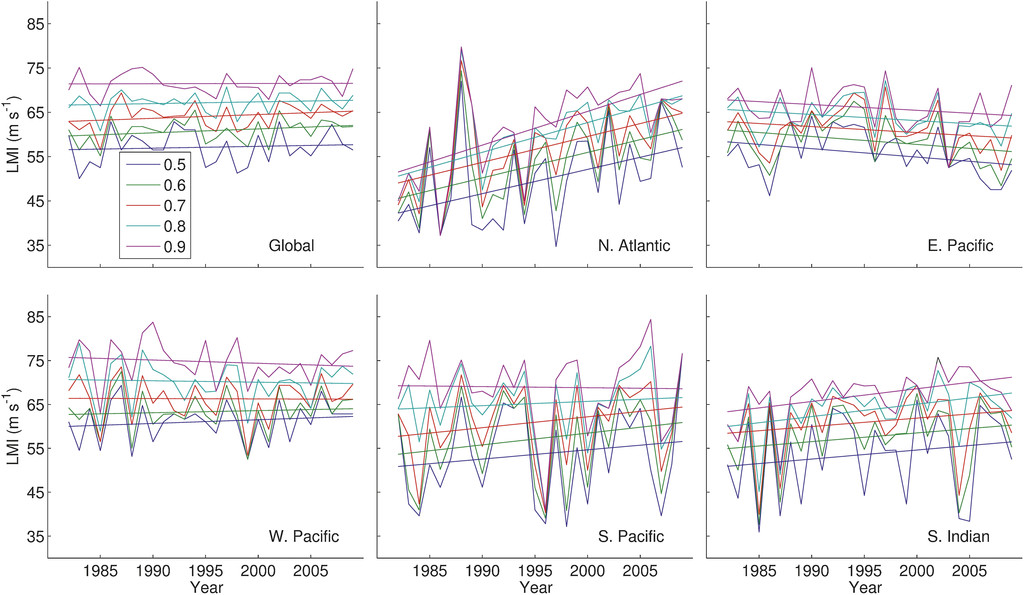
\includegraphics[width=\textwidth]{trends_lmi_kossin_2013.jpg}
    \caption{Évolution temporelle de l'intensité maximale sur le cycle de vie des TC (\textit{lifecycle maximum intensity}, LMI) entre 1982 et 2009, présentée
        par les quantiles entre \num{0.5} et \num{0.9} de la distribution associée et leur tendances linéaires. Intensités calculées avec une base de données
        homogénéisée de l'intensité construite à partir d'images satellites \hbox{HURSAT} (\textit{Hurricane Satellite}) auxquelles est appliquée la technique
        de Dvorak avancée (\textit{Advanced Dvorak Technique}, ADT, \cite{olander_advanced_2007}). Figure issue de \hbox{\cite{kossin_trend_2013}}}
    \label{fig:observed_trends_lmi}
\end{figure}

En dépit de toutes ces difficultés, la mise en commun des données issues de chaque centre spécialisé en un fichier unique est précisément l'objectif de la base
de données IBTrACS (\textit{International Best Track Archive for Climate Stewardship}, \cite{knapp_international_2010}). Bien qu'IBTrACS puisse être moins
détaillé que certaines bases de données locales, comme par exemple HURDAT2 pour l'océan Atlantique \parencite{landsea_atlantic_2013} qui fournit une information
sur la taille des cyclones à travers l'étendue maximale des vents à \num{34}, \num{50} et \SI{64}{\knot} dans les quatre quadrants autour du centre du système,
elle possède donc néanmoins la qualité de couvrir tous les bassins géographiques et fournit également une grande quantité de méta données permettant de filtrer
au mieux les informations. Pour cette raison, IBTrACS est la base de données observationnelle qui est utilisée à travers tout ce document. Il demeure que toutes
les sources d'hétérogénéité mentionnées, spatiales comme temporelles, y compris la rupture causée par l'avènement de l'ère satellitaire, constituent autant de
limites à l'analyse de tendances historiques de l'activité cyclonique tropicale.

\begin{figure}[tb]
    \centering
    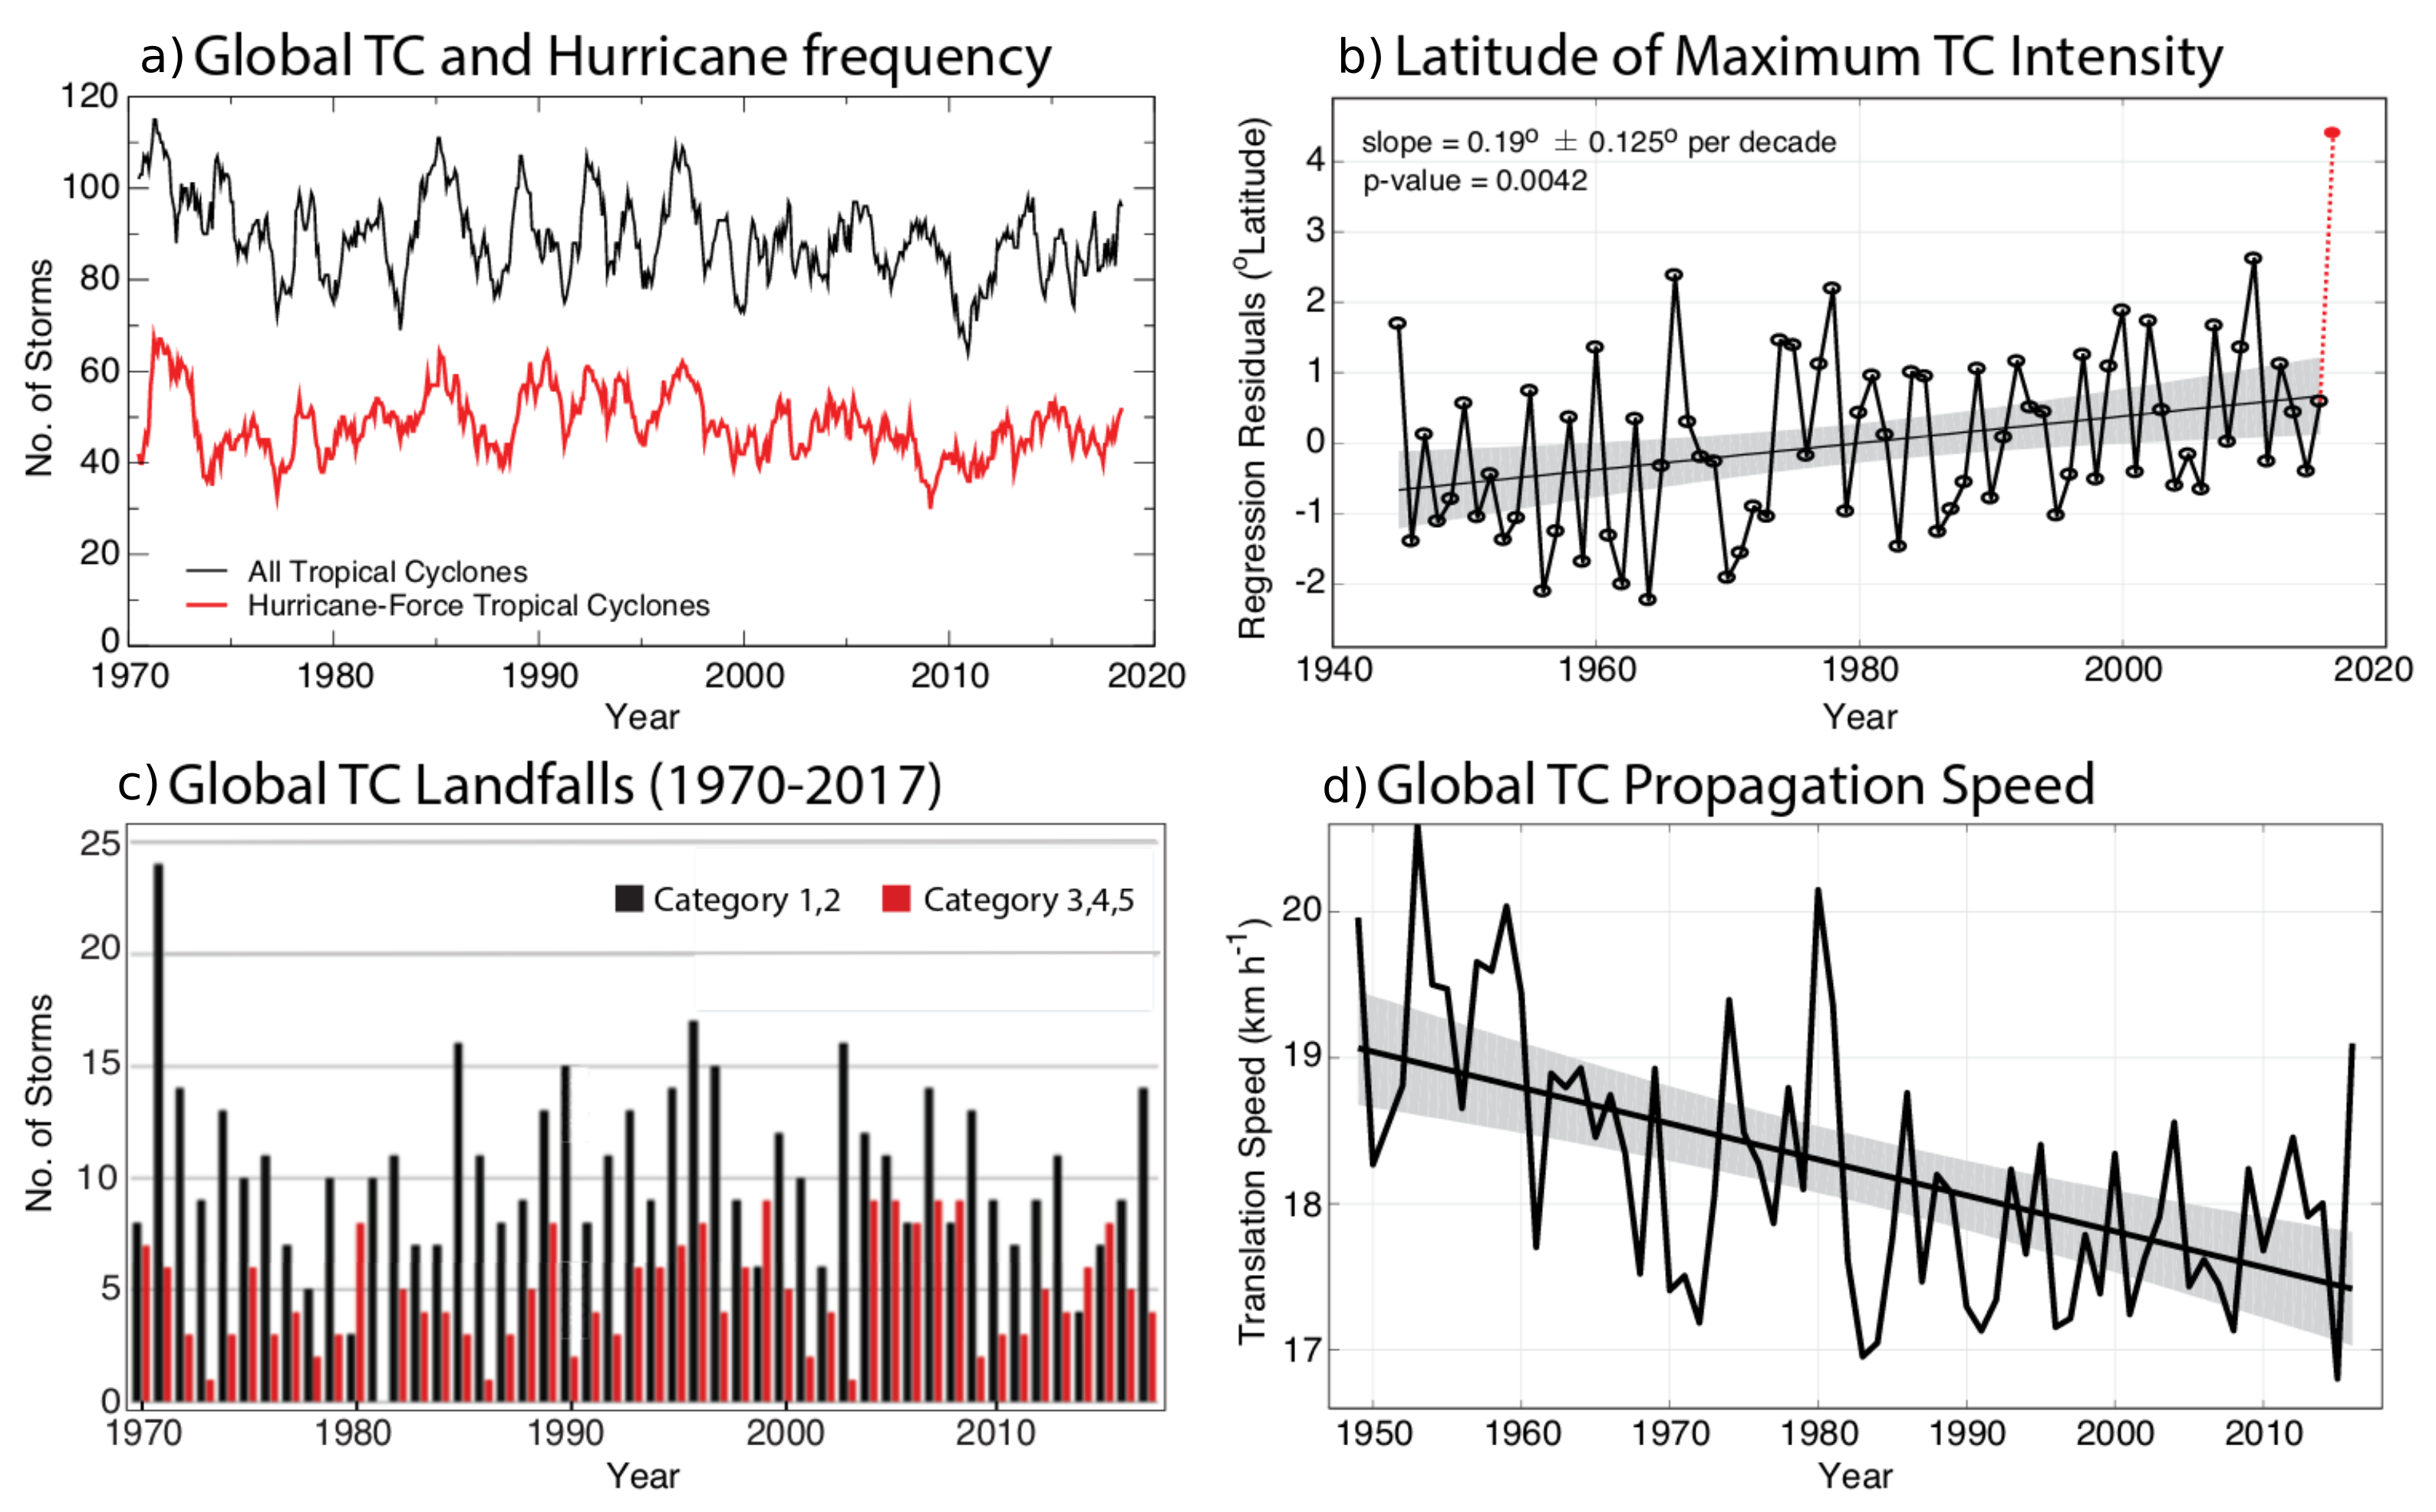
\includegraphics[width=\textwidth]{trends_freq_lat_land_speed_kossin_2019.png}
    \caption{\textbf{(a)} Fréquence globale annuelle des tempêtes tropicales (\SI{34}{\knot}) en noir et des TC atteignant au moins la catégorie 1 en rouge
        (\SI{64}{\knot}) entre 1970 et Mai 2018 et sous forme de somme glissante sur 12 mois \parencite{maue_recent_2011}. \textbf{(b)} Évolution annuelle de la
        moyenne des latitudes auxquelles l'intensité maximale est atteinte dans le bassin WPac, après retranchement de l'influence des modes de variabilité El Niño et de
        l'oscillation décennale du Pacifique par régression linéaire, et intervalle de confiance à \SI{95}{\percent} \parencite{kossin_comment_2018}. \textbf{(c)}
        Fréquence annuelle des TC touchant terre pour les catégories \num{1} et \num{2} (noir) et de \num{3} à \num{5} (rouge) entre 1970 et 2016
        \parencite{weinkle_historical_2012}. \textbf{(d)} Vitesse moyenne globale de translation des TC entre 1949 et 2016 et son intervalle de confiance à
        \SI{95}{\percent} \hbox{\parencite{kossin_global_2018}}. Les encadrés (a) et (c) ont été mis à jour par leurs auteurs respectifs dans le cadre de
        \cite{knutson_tropical_2019}, étude dont sont issues ces quatre figures.}
    \label{fig:observed_trends_other}
\end{figure}

Une des tendances historiques les plus facilement détectable concerne l'intensité des cyclones tropicaux. À partir d'une base de données construite dans un
soucis d'homogénéisation spatiale et temporelle de l'intensité observée des TC issus des best tracks, la \cref{fig:observed_trends_lmi} présente les tendances
dans les quantiles de la distribution de l'intensité maximale des cyclones sur la période \num{1982}~--~\num{2009} et fait apparaître une tendance positive
faible à l'échelle globale, indiquant donc un changement vers des systèmes plus forts \parencite{kossin_trend_2013}. Cette tendance globale cache toutefois de
fortes disparités régionales, avec notamment une très forte tendance positive dans le NAtl ---~pouvant s'expliquer au moins en partie par l'augmentation
constatée des SST dans la région due à la phase ascendante actuelle de l'oscillation atlantique multidécénnale (OAM, ou AMO en anglais)
\parencite{ting_forced_2009}~--- et au contraire une diminution de l'intensité dans le bassin EPac. En répétant l'exercice avec des données étendues jusqu'en
\num{2017}, \cite{kossin_global_2020} confirme une tendance à la hausse dans la probabilité de dépassement des TC majeurs et établit une significativité
supérieure à \SI{95}{\percent} pour l'échelle globale, et de \SI{99}{\percent} pour le NAtl. Parmi les autres bassins, seul le SInd présente une significativité
d'au moins \SI{90}{\percent}. Cette propension vers des cyclones plus intenses est accompagnée d'une augmentation du taux d'intensification des TC ainsi que de
la fréquence de cas d'intensification rapide \parencite{balaguru_increasing_2018,kishtawal_tropical_2012}. Dans le bassin WPac, si aucune tendance très nette
dans l'évolution annuelle du LMI ne se dégage, il existe néanmoins une tendance positive statistiquement significative dans la latitude moyenne auxquelles les
TC atteignent leur maximum d'intensité (\cref{fig:observed_trends_other}, encadré \textbf{b}, \hbox{\cite{kossin_comment_2018}}), avec un degré de confiance
jugé faible quant au  fait que cette tendance puisse être attribuable à des forçages anthropiques \parencite{knutson_tropical_2019}. Le décalage vers les pôles
de l'intensité maximale des TC est également détectable à l'échelle globale \parencite{kossin_poleward_2014}. Il est considéré que la fréquence d'occurrence
globale des cyclones tropicaux ---~présentée sur la \cref{fig:observed_trends_other}, encadré \textbf{a}~--- ne présente pas de tendance à long terme
détectable, mais qu'il existe cependant une augmentation de l'activité dans le bassin NAtl depuis \num{1995}
\parencite{webster_changes_2005,maue_recent_2011,wang_climate_2010,seneviratne_weather_2021}. Néanmoins l'étude plus récente de \cite{klotzbach_trends_2022}
portant sur la période \num{1990}~--~\num{2021} établit une tendance globale à la baisse, portée par une diminution de l'activité dans le WPac plus importante
que la hausse du NAtl, et qui serait liée à une tendance à un état de base plus proche de La Niña depuis \num{1990}, c'est à dire marquée par une anomalie
froide des SST équatoriales dans le Pacifique centre. Par ailleurs, si la quantité de TC touchant terre ne présente pas de tendance globalement, une tendance à
la baisse est reconnue en Australie de l'est depuis la fin du \num{19}\ieme~siècle \parencite{knutson_tropical_2019,callaghan_variability_2011}. Enfin,
\cite{kossin_global_2018,kossin_reply_2019} a établi une tendance significative à une baisse de la vitesse de translation des TC, présentée sur la
\cref{fig:observed_trends_other}, encadré \textbf{d} et évaluée à \SI{10}{\percent} entre \num{1949} et \num{2016}. Un ralentissement des TC pourrait avoir des
conséquences désastreuses dans la mesure où ces derniers aurait alors plus de temps pour causer des dégâts dans les zones habitées. Si la confiance accordée à
la détectabilité de cette tendance est jugée bonne \parencite{knutson_tropical_2019,seneviratne_weather_2021}, il est à souligner que ce résultat est néanmoins
contesté, notamment par \cite{lanzante_uncertainties_2019,moon_climate_2019} qui estiment que cette tendance pourrait être causée par l'hétérogénéité des
données, et plus spécifiquement par l'introduction de données satellitaire à partir de \num{1965}.

\subsection{Les modèles de climat}

Le terme \textquote{modèle de climat} est souvent utilisé comme un terme parapluie puisqu'il peut se référer aussi bien à un ensemble de modèles fonctionnant en
configuration couplée, c'est à dire de façon à ce que chaque composante puisse interagir avec les autres afin de mieux simuler les rétroactions, comme il peut
se référer à une seule composante, celle-ci étant en général la composante atmosphérique, à fortiori lorsqu'il s'agit d'étudier les cyclones tropicaux. Dans cet
ouvrage, sauf indication contraire, c'est ce second usage du terme qui sera privilégié. Les modèles de climat, ou modèles de circulation atmosphériques, sont
des programmes informatiques qui simulent l'évolution de variables atmosphériques (température, pression, humidité...) à un pas de temps régulier, sur chacune
des mailles composant la grille du modèle, et ce en suivant les lois de la dynamique et de la physique atmosphérique. La partie dynamique du modèle consiste en
la résolution à chaque pas de temps d'un jeu d'équations différentielles décrivant la circulation atmosphérique, tandis que la physique et les processus prenant
place à une échelle caractéristique plus petite que la taille d'une maille sont paramétrisées. Les modèles de climat peuvent soit simuler l'atmosphère sur
l'entièreté du globe, auquel cas il s'agit de modèles de circulation globaux (\textit{Global Circulation Model}, GCM), ou bien ne simuler qu'un domaine
spécifique~---~il s'agit alors de modèles à aire limitée, ou modèles régionaux (\textit{Regional Circulation Model}, RCM).
%
\begin{figure}[t]
    \centering
    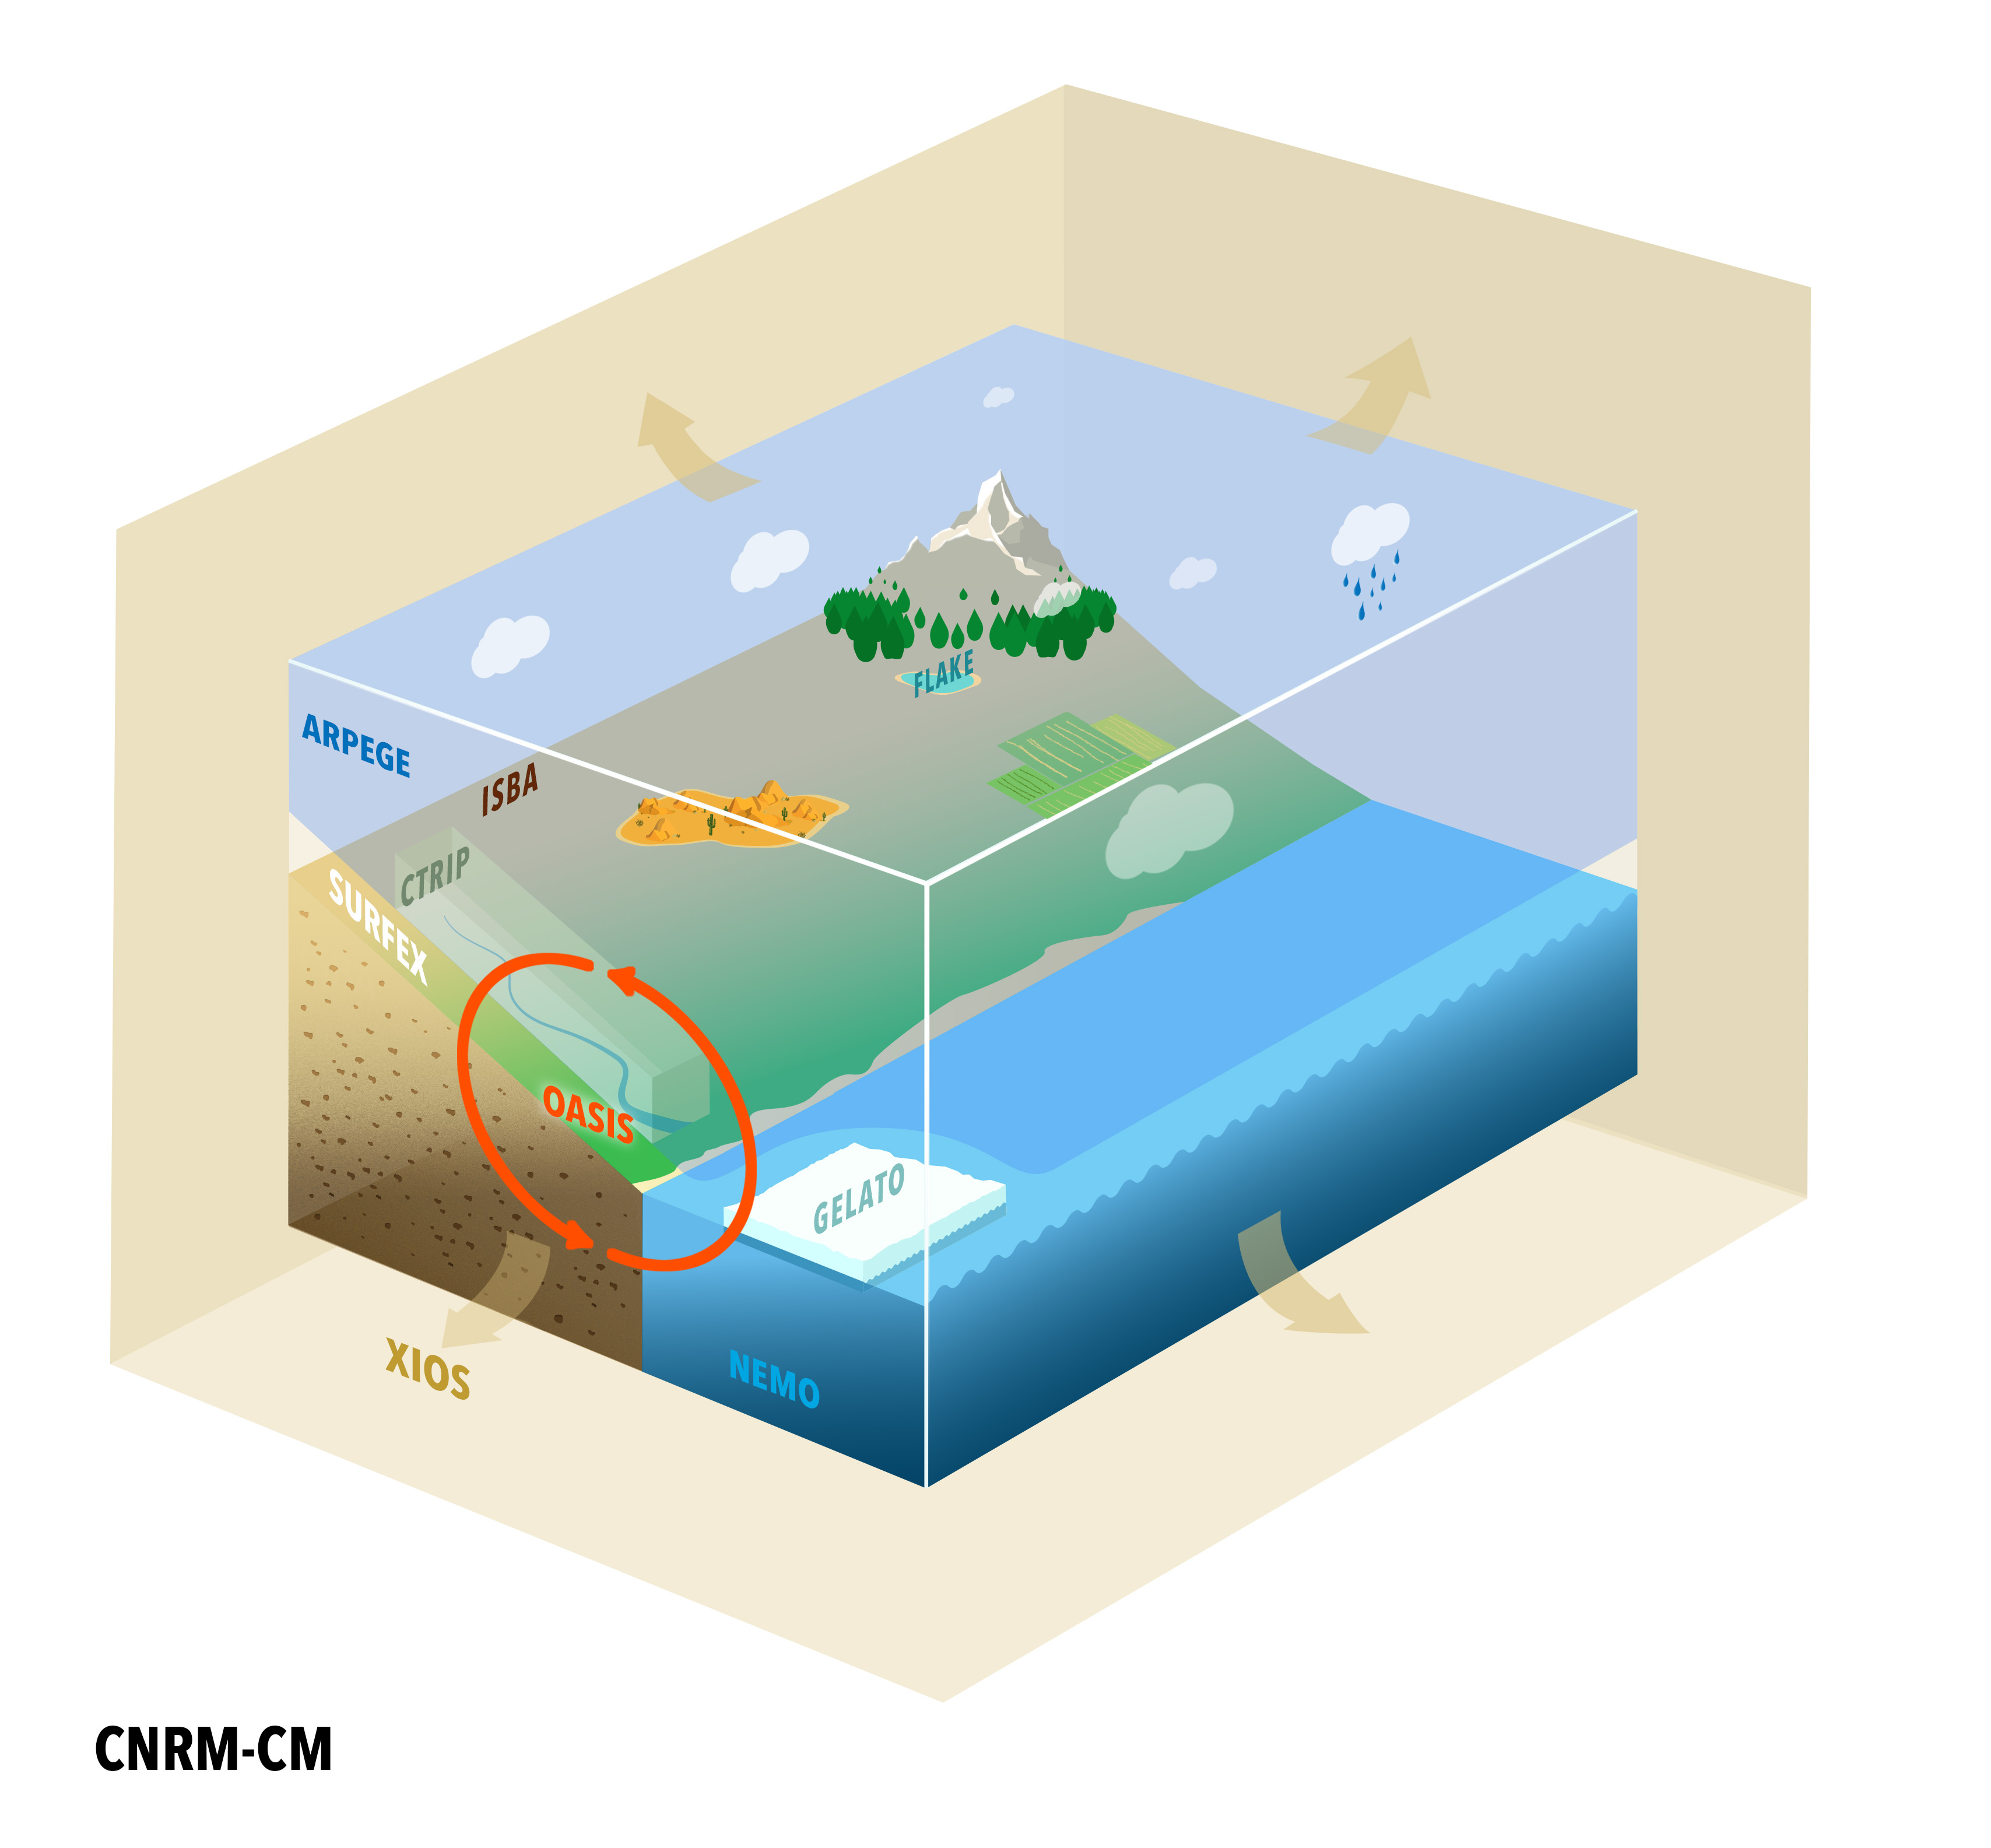
\includegraphics[width=\textwidth]{cnrm-cm6.jpg}
    \caption{Représentation schématique du modèle couplé océan-atmosphère CNRM-CM6-1. \hbox{ARPEGE} constitue la composante atmosphérique de CNRM-CM, ainsi que
    celle du modèle système-terre CNRM-ESM \parencite{seferian_evaluation_2019}. Illustration issue de \cite{voldoire_evaluation_2019}.}
    \label{fig:cnrm-cm6}
\end{figure}
%
Au CNRM, le modèle atmosphérique global est nommé ARPEGE-Climat \parencite[Action de Recherche Petite Échelle Grande Échelle,][]{deque_arpege_1994} de  et est
dérivé du modèle de prévision numérique du temps ARPEGE/IFS \parencite[\textit{Integrated Forecast System},][]{courtier_arpege_1991}, développé conjointement
par Météo-France et le CEPMMT. En tant que composante atmosphérique dans le modèle couplé océan-atmosphère \nolinebreak CNRM-CM6-1
\parencite{voldoire_evaluation_2019}, ARPEGE est doté d'une résolution horizontale d'environ \ang{1.4} à l'équateur, ou approximativement \km{140}, et \num{91}
niveaux verticaux. Cela situe donc ARPEGE à peu près dans la moyenne des modèles globaux modernes puisque la résolution des modèles atmosphériques ayant pris
part au sixième et plus récent exercice d'intercomparaison des modèles couplés (\textit{Coupled Model Intercomparison Project}, CMIP, ici CMIP6)
\parencite{eyring_overview_2016} varie entre \km{80} et \km{250} \parencite[][Tableau AII.5]{ipcc_annex_2021}. Une version dite haute-résolution du modèle
ARPEGE existe néanmoins et est utilisée dans le modèle couplé CNRM-CM6-1-HR \parencite{saint-martin_tracking_2021}, participant au projet d'intercomparaison des
modèles haute résolution (\textit{High Resolution Model Intercomparison Project}, HighResMIP) \parencite{haarsma_high_2016} et fonctionnant à une une résolution
horizontale de \km{50} ---~les autre modèles participants se situant entre \km{20} et \km{80} \parencite[][Tableau AII.6]{ipcc_annex_2021}. Ainsi, de manière
générale un GCM disposant d'une résolution horizontale plus fine que \km{100} peut être considéré comme un modèle à haute résolution.
%
\begin{figure}[t]
    \centering
    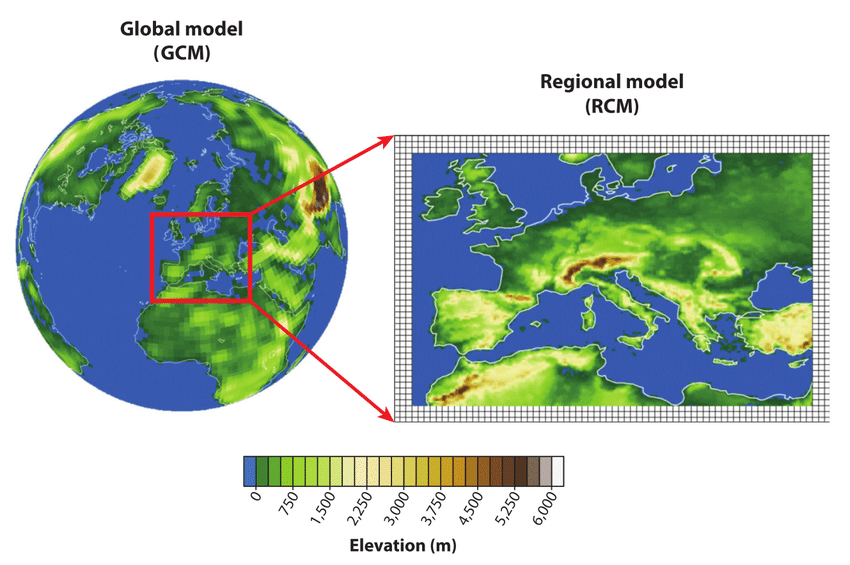
\includegraphics[width=0.8\textwidth]{dynamical_downscaling.png}
    \caption{Illustration schématique du raffinement en résolution permis par l'utilisation d'un modèle à aire limitée. Ce dernier nécessite que des
    conditions limites lui soient fournies aux bords du domaine simulé à chaque pas de temps, le plus souvent par l'intermédiaire d'un GCM, à travers une zone
    tampon, ici représentée par le maillage entourant le domaine du RCM. Illustration issue de \hbox{\cite{giorgi_regional_2015}}.}
    \label{fig:dynamical_downscaling}
\end{figure}

La résolution d'un modèle est déterminante dans sa capacité à simuler une activité cyclonique réaliste \parencite{roberts_impact_2020}, aussi bien pour ce qui
est de la fréquence d'occurrence que pour l'intensité des systèmes simulés, puisqu'il est estimé qu'un modèle doté d'une résolution plus large que \km{25} ne
saurait produire une quantité réaliste de cyclones de catégorie 4 sur l'échelle de Saffir-Simpson \parencite{davis_resolving_2018}, ce qui laisse entendre que
la majorité des GCM à haute résolution n'en sont donc pas capables. Il est cependant possible d'accroître la résolution des modèles de circulation
atmosphérique. Une des solutions consiste à utiliser un modèle dit à aire limitée (RCM). En ne simulant l'évolution de l'atmosphère que sur un domaine
restreint, ces derniers sont en mesure d'opérer à des résolutions nettement plus fines avec des temps de calcul raisonnables, typiquement de l'ordre de \km{25}
sur des bassins cycloniques \parencite{torres-alavez_future_2021}. Toutefois, un RCM ne peut pas fonctionner de manière purement autonome car il a besoin de
connaître l'état de l'atmosphère aux limites de son domaine. Ces informations sont fournies par un autre modèle qui l'englobe, souvent un GCM, ou parfois même
un autre RCM si le saut de résolution est trop important (constituant donc une chaîne à trois modèles). La cohabitation nécessaire entre le RCM et son GCM
forceur n'est pas sans inconvénients, car le RCM est alors très sensible à ces conditions limites \parencite{wu_estimating_2005} et donc au choix du GCM. La
réciproque n'est cependant pas vraie puisque le RCM ne peut pas communiquer en retour au GCM, ce qui peut donner lieu à des incohérences si la simulation du RCM
s'éloigne trop des champs fournis par la grande échelle du fait des différences dans la dynamique et la physique des deux composants. Des techniques existent
pour imposer cette cohérence \parencite{storch_spectral_2000,biner_nesting_2000}, mais des doutes subsistent sur le bienfondé de la démarche, puisque cela
pourrait revenir à inhiber la capacité du RCM à produire de la valeur ajoutée \parencite{alexandru_sensitivity_2009,separovic_impact_2012,omrani_spectral_2012}
dans la mesure où il est permis de penser que c'est la liberté propre du modèle qui est à l'origine des détails de fine échelle réalistes et de leur évolution,
celles-ci étant précisément issues de son implémentation et donc de ses différences avec le GCM forceur. Le gain de résolution apportée par l'utilisation de
modèles à aire limitée est donc contrebalancé par l'introduction de nouvelles incertitudes et difficultés associées.
%
\begin{figure}[tb]
    \centering
    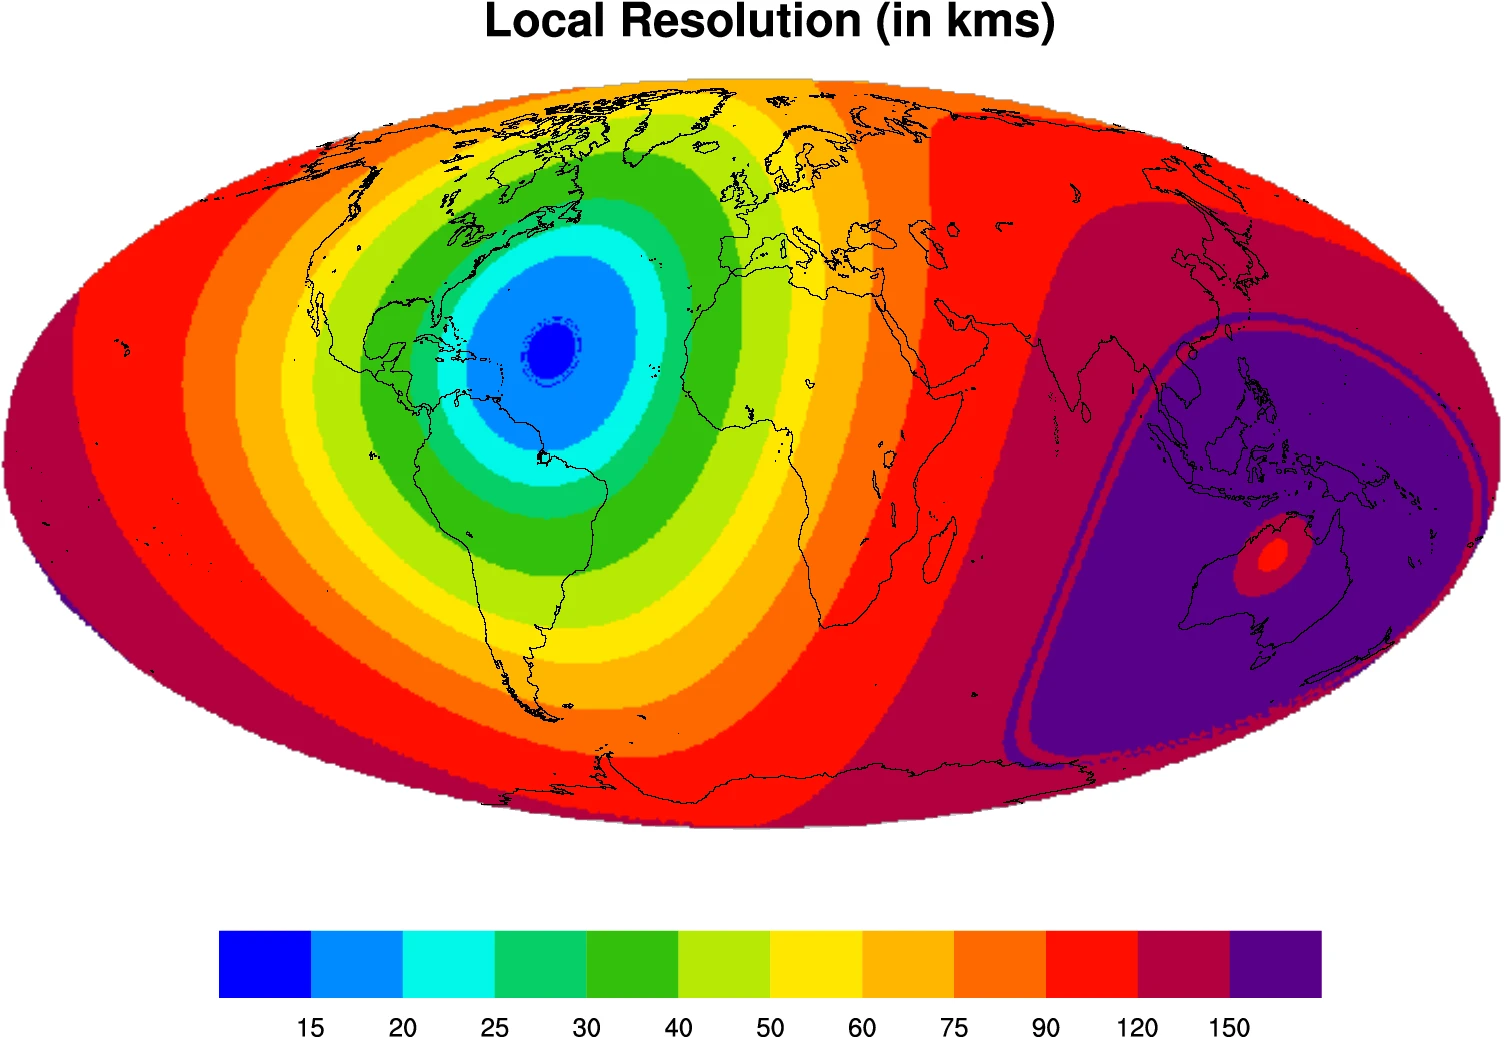
\includegraphics[width=0.8\textwidth]{grille_arpege_stretchee_C3AF.png}
    \caption{Exemple d'utilisation de la grille ARPEGE dans sa configuration tournée étirée, où le pôle est positionné sur une région d'intérêt et un facteur
    d'étirement est appliqué pour y augmenter localement la résolution (ici égal à \num{3.5}) au détriment de l'antipode. Figure issue de
    \cite{chauvin_future_2020}.}
    \label{fig:rotated_streched}
\end{figure}

Comme alternative aux modèles à aire limitée pour bénéficier d'une résolution accrue, le modèle ARPEGE dispose de la capacité à déformer sa grille horizontale
de telle sorte à augmenter significativement sa résolution sur une région d'intérêt \parencite{courtier_global_1988}. Pour ce faire, la position du pôle est
centrée sur la région désirée avant d'appliquer la transformation de \cite{schmidt_variable_1977} avec un facteur d'étirement $c$. Si \cite{caian_limits_1997}
ont montré que la précision du modèle demeurait bonne jusqu'à un facteur $c=7$ ---~au delà de quoi l'usage d'un RCM peut être préférable~--- l'étirement est en
pratique souvent limité à \num{3.5}, valeur pour laquelle le modèle a initialement été validé pour la prévision opérationnelle du temps à court terme
\parencite{benichou_validation_1992}. Cette capacité permet à ARPEGE d'atteindre localement jusqu'à \km{14} de résolution à l'emplacement du pôle, avec un
minimum de \km{35} sur un bassin comme le NAtl \parencite[][c.f \cref{fig:rotated_streched}]{chauvin_future_2020} et de \km{50} sur un bassin plus large comme
le SInd \parencite{cattiaux_projected_2020}\footnote{Dans \cite{cattiaux_projected_2020}, le pôle est placé de telle sorte à maximiser la résolution autour de l'île
de La Réunion, au détriment des côtes Est de l'Australie. Il serait sinon possible de garantir une résolution inférieure à \km{40} sur l'ensemble du bassin.}.
La spécificité de sa grille place ARPEGE dans le cercle très restreint des GCM à résolution variable, puisqu'ils sont au nombre de cinq
\parencite{mcgregor_recent_2013}, et ARPEGE est le premier d'entre eux à avoir été utilisé pour réaliser des simulations climatiques
\parencite{deque_high_1995}. Cette technique a été maintes fois employée pour l'étude des cyclones tropicaux
\parencite{chauvin_response_2006,chauvin_atlantic_2017,chauvin_future_2020,daloz_impact_2012,cattiaux_projected_2020}, y compris en changement climatique, et
permet donc de profiter des bénéfices de la haute résolution sans les inconvénients des modèles à aire limitée.

\subsection{Les cyclones dans les modèles de climat}

\cite{manabe_tropical_1970} ont pour la première fois observé, dans une simulation produite par un GCM doté d'une résolution horizontale de \km{417} à
l'équateur, des vortex pouvant s'apparenter à des cyclones tropicaux sous la forme de très larges dépressions atmosphériques de l'ordre de \km{2000} à \km{3000}
de diamètre dans le Sud-ouest de l'océan indien et dans le Pacifique Sud, à des emplacements correspondant aux zones de formation des TC de l'hémisphère sud
identifiées par \cite{gray_global_1968} (voir aussi \cref{fig:produit_ingredients}). Limitées par la résolution du modèle, les dépressions tropicales de
\cite{manabe_tropical_1970} atteignent une vitesse de vent maximale de \ms{20}, soit un stade de tempête tropicale, et ne peuvent pas s'intensifier au delà.
\cite{bengtsson_simulation_1982} ont ensuite proposé une étude plus approfondie des divers stades de développement des TC simulés dans le modèle opérationnel du
CEP, à environ \km{200} de résolution, dans lequel ces objets atteignent un vent tangentiel maximum de \ms{25}. Outre la taille et l'intensité des systèmes
simulés, et malgré une structure interne réaliste lorsque les systèmes sont pleinement développés, \cite{mcbride_comments_1984} souligne plusieurs autres
différences clefs entre les simulations et les TC observés, notamment pendant les étapes de formation et d'intensification, marquées par une très forte activité
convective néanmoins accompagnée d'une absence de cœur chaud et d'une faible vorticité. L'auteur souligne également le lien exacerbé entre la SST et l'activité
simulée, en dépit des autres facteurs favorables à la cyclogénèse identifiés par \cite{gray_tropical_1975} (voir \cref{sec:conditions_cyclogenese}), et
qui explique la répartition spatiale et temporelle imparfaite de l'activité simulée. La faible résolution des GCM et la paramétrisation nécessaire de la
microphysique propre aux TC en résultant font qu'il est très difficile de simuler correctement ces systèmes complexes, si bien que la dénomination de HTV
(\textit{Hurricane-Type Vortices}) est parfois préférée pour les désigner
\parencite{bengtsson_simulation_1982,bengtsson_hurricanetype_1995,chauvin_response_2006}.

\begin{figure}[htbp]
    \centering
    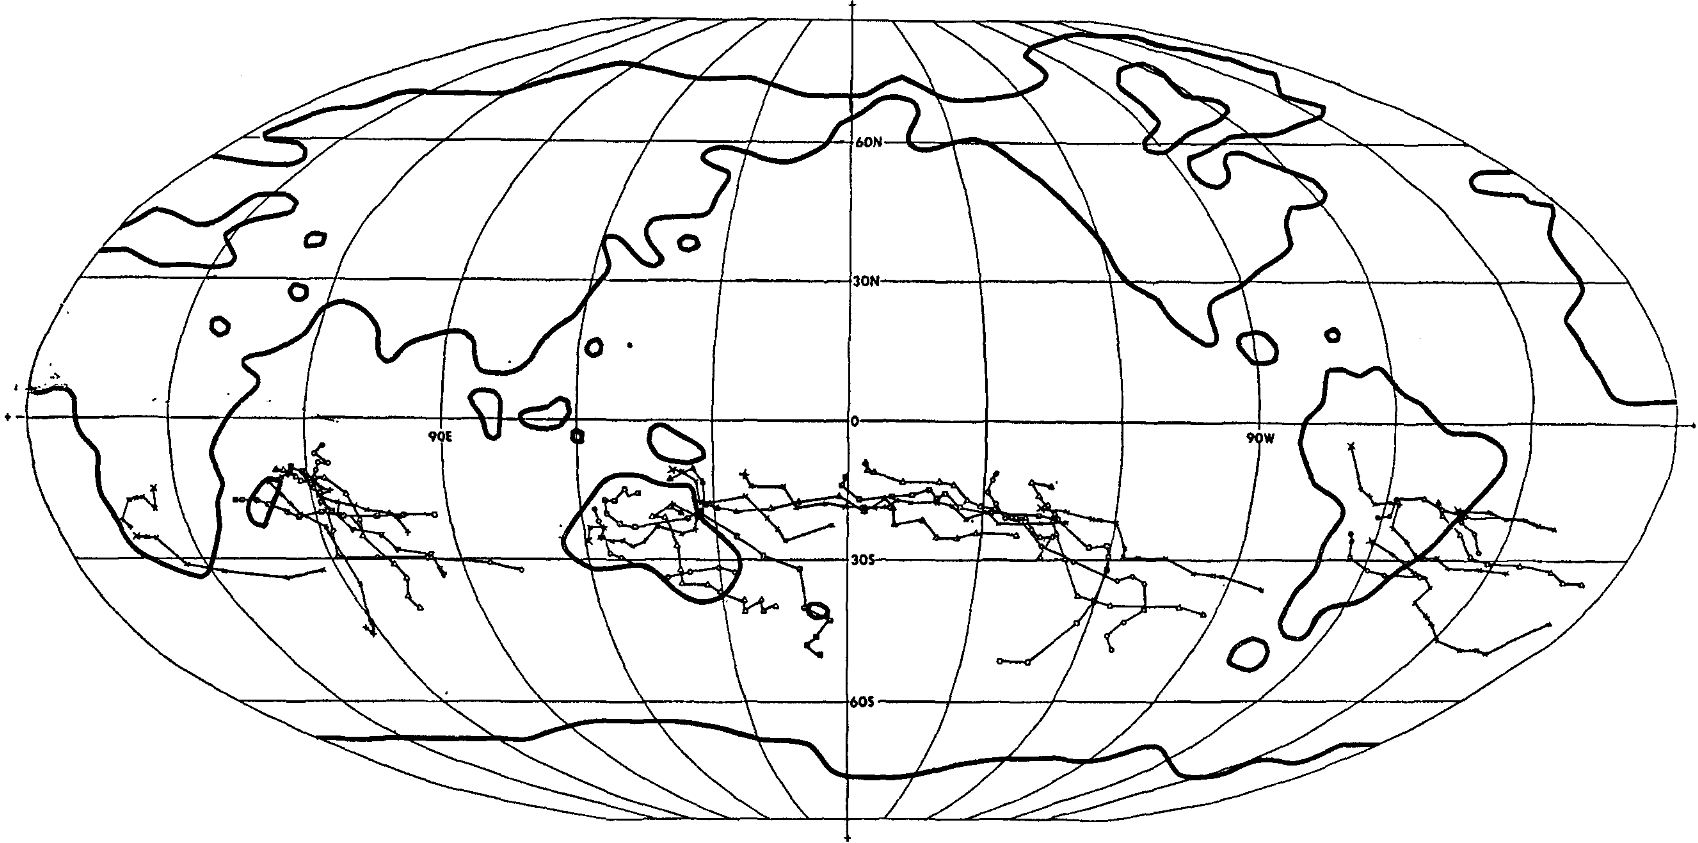
\includegraphics[width=0.9\textwidth]{manabe_1970_tracks_screenshot.png}
    \caption{Trajectoires des HTV détectés par \cite{manabe_tropical_1970}, caractérisés par une dépression centrale d'au moins \hPa{2}. Les croix désignent les
        premières positions des HTV, tandis que les symboles représentent leurs positions respectives avec un intervalle de \SI{24}{\hour}.}
    \label{fig:tracks_manabe}
\end{figure}

\cite{broccoli_can_1990} ont ensuite pour la première fois essayé d'utiliser un modèle de climat pour étudier l'influence du changement climatique sur
l'activité cyclonique, en analysant les HTV dans le modèle du GFDL (\textit{Geophysical Fluid Dynamics Laboratory}) via des expériences à deux résolutions
différentes (\ang{4.5}\times\ang{7.5} et \ang{2.25}\times\ang{3.75}, en latitude et longitude, respectivement), \num{9} niveaux verticaux, avec et sans
rétro-actions nuageuses et dans lesquelles la concentration en \ce{CO2} est doublée. Ils notèrent ainsi un changement à la baisse en
\ensuremath{2\times\ce{CO2}} dans la simulation avec rétro-action nuageuse, et au contraire une augmentation lorsque la nébulosité est prescrite, indépendamment
de la résolution utilisée. Ces expériences, bien que peu concluantes, validèrent le principe de l'utilisation de GCM pour l'étude des TC en changement
climatique. \cite{haarsma_tropical_1993,bengtsson_will_1996} procédèrent à de nouvelles expériences en \ensuremath{2\times\ce{CO2}} et notèrent une augmentation
relative de la fréquence des cyclones les plus forts. \cite{bengtsson_will_1996} observa par ailleurs pour la première fois une réduction de l'activité dans la
simulation \ensuremath{2\times\ce{CO2}}. Une réduction de l'activité cyclonique accompagnée d'une augmentation relative de la fréquence d'occurrence des TC les
plus forts constitue un signal robuste de réponse au changement climatique encore aujourd'hui \parencite[][voir
\cref{sec:projections_futures}]{walsh_tropical_2016,camargo_tropical_2016,knutson_tropical_2010,christensen_climate_2013,seneviratne_weather_2021}. À la même
époque, \cite{bengtsson_hurricanetype_1995} notèrent une forte variabilité inter-annuelle de l'activité cyclonique dans leurs simulations, en dépit du fait que
des SST climatologiques ---~donc dénuées de cette variabilité~--- furent prescrites, et établirent un lien entre l'activité simulée et des modes de circulation
de grande échelle, s'affranchissant ainsi du trop fort lien entre SST et cyclogénèse des HTV dans les premières expériences. Leurs travaux montrèrent également
un lien clair entre la résolution du modèle d'une part, et l'intensité ainsi que le réalisme de la structure interne des HTV d'autre part.

\begin{figure}[tb]
    \centering
    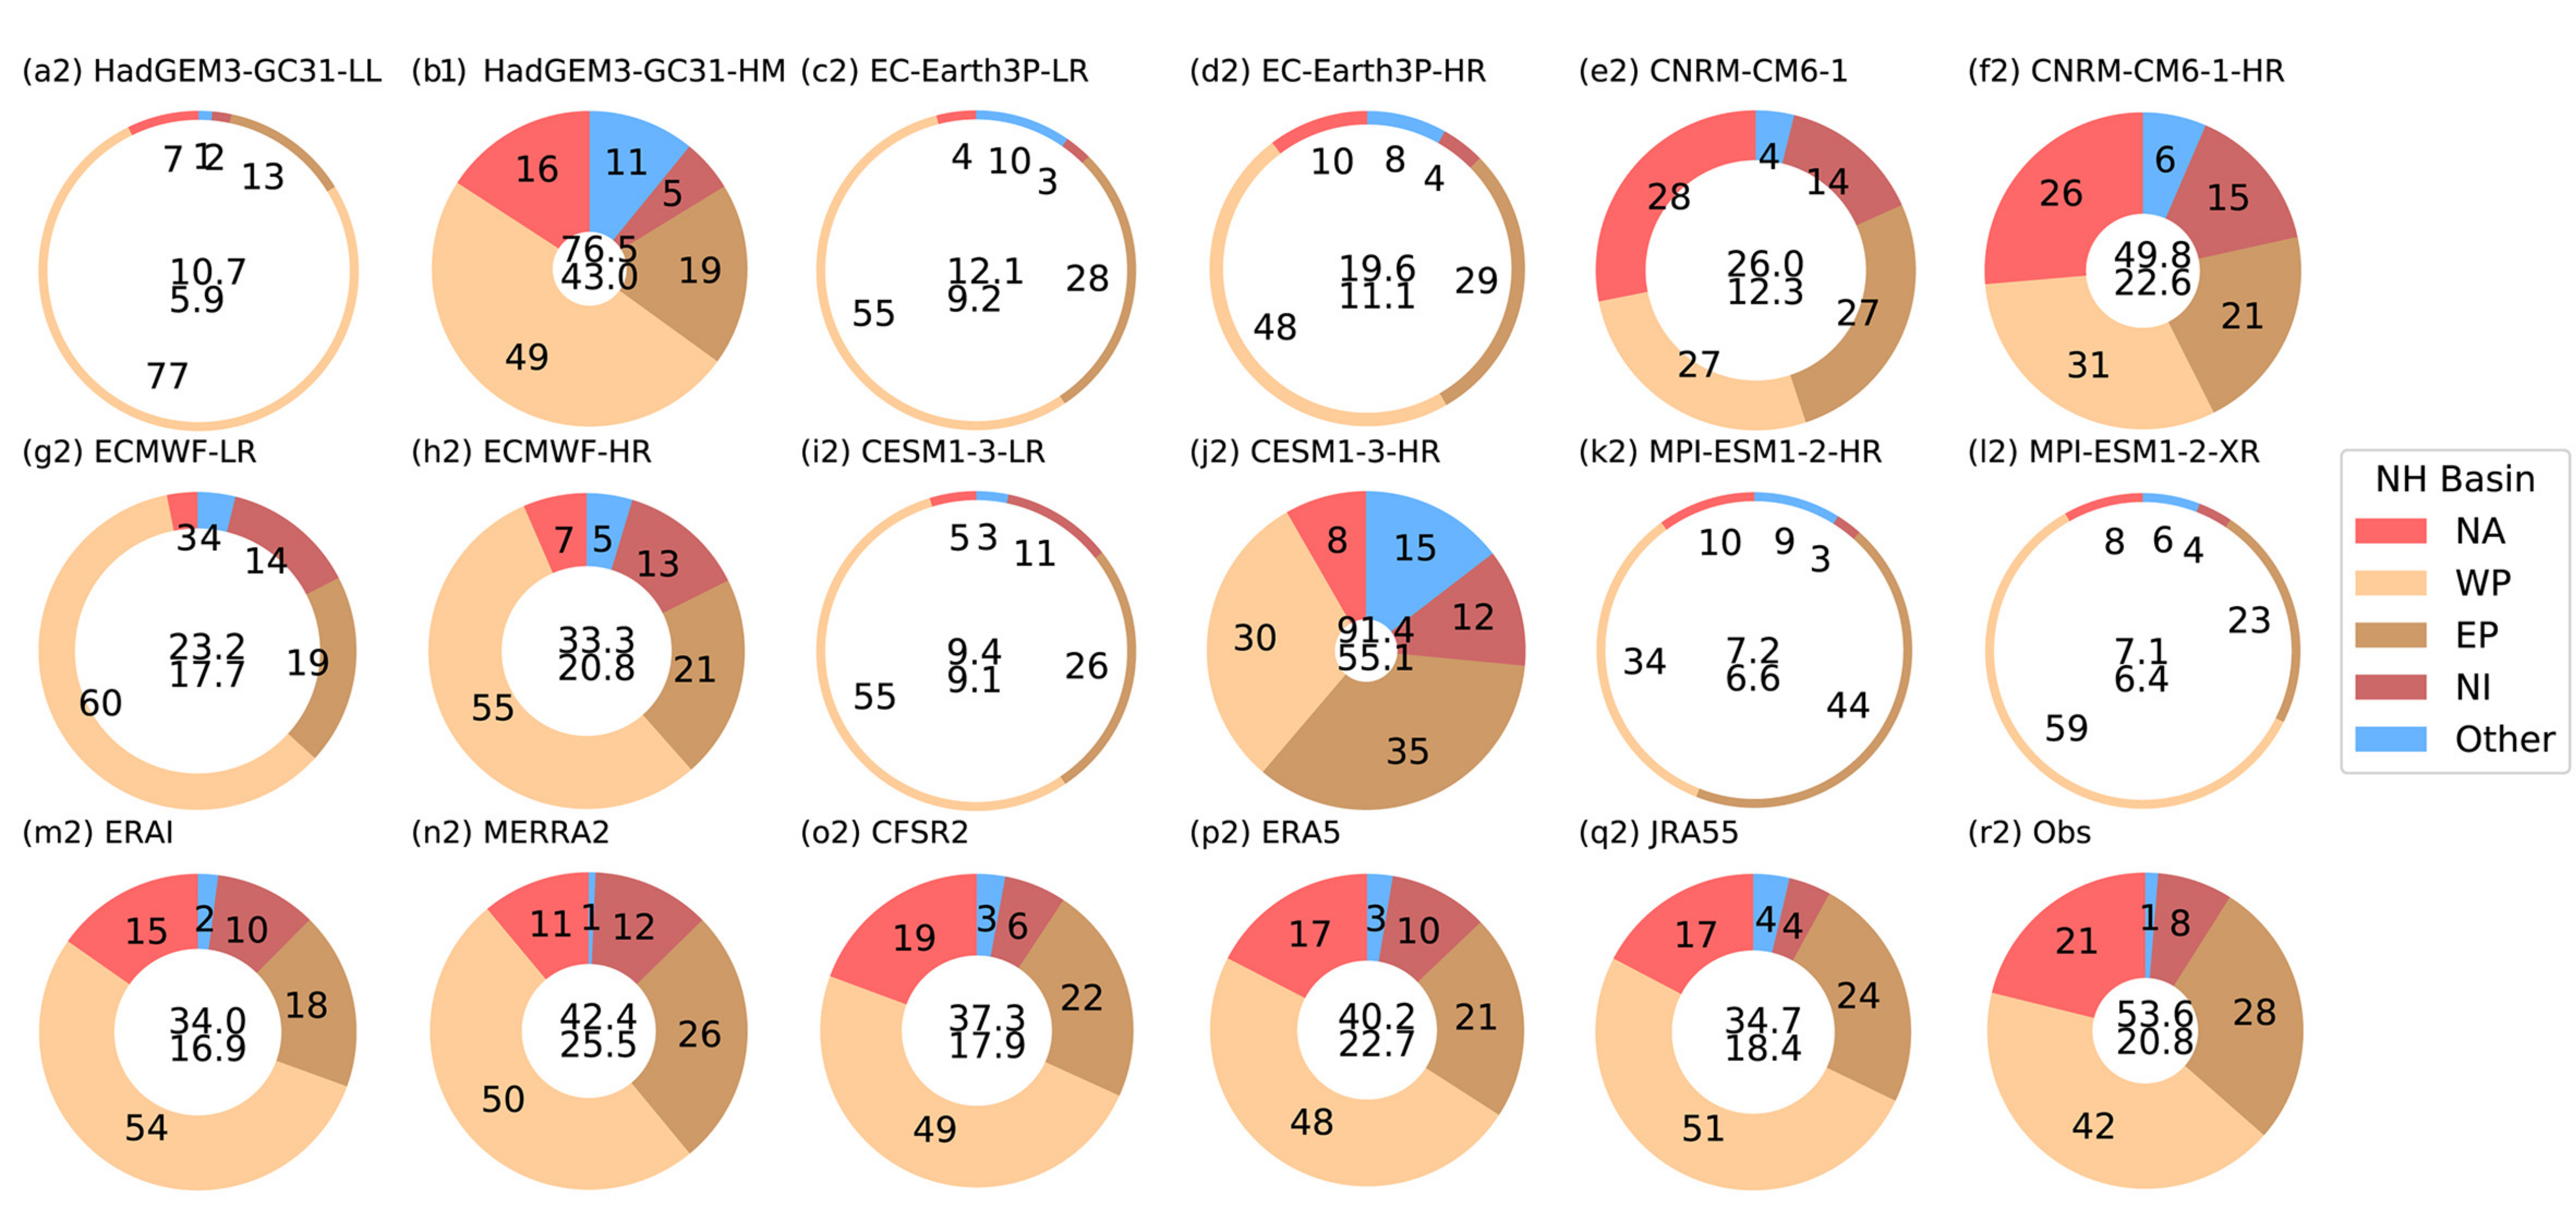
\includegraphics[width=\textwidth]{roberts_projected_2020_TE_coupled.png}
    \caption{Fréquence annuelle moyenne du nombre de TC dans des simulations historiques couplées océan-atmosphère HighResMIP (tiers 2) sur la période
        \num{1974}~--~\num{2014} (deux premières lignes) ainsi que pour cinq réanalyses et dans les observations (dernière ligne). Moyenne annuelle entre Mai et
        Novembre dans l'hémisphère nord et Octobre~--~Mai dans l'hémisphère sud. Les modèles couplés sont par paire basse / haute résolution. Les deux valeurs
        centrales de chaque disque présentent la moyenne dans les deux hémisphères et les tranches de couleur présentent le pourcentage de HTV de l'hémisphère
        nord pour chaque bassin d'activité. L'épaisseur des disques est calibrée sur le nombre annuel de TC observé dans l'hémisphère nord. Figure issue de
        \hbox{\cite{roberts_projected_2020}}.}
        \label{fig:NTC_HighResMIP}
\end{figure}
\begin{figure}[tb]
    \centering
    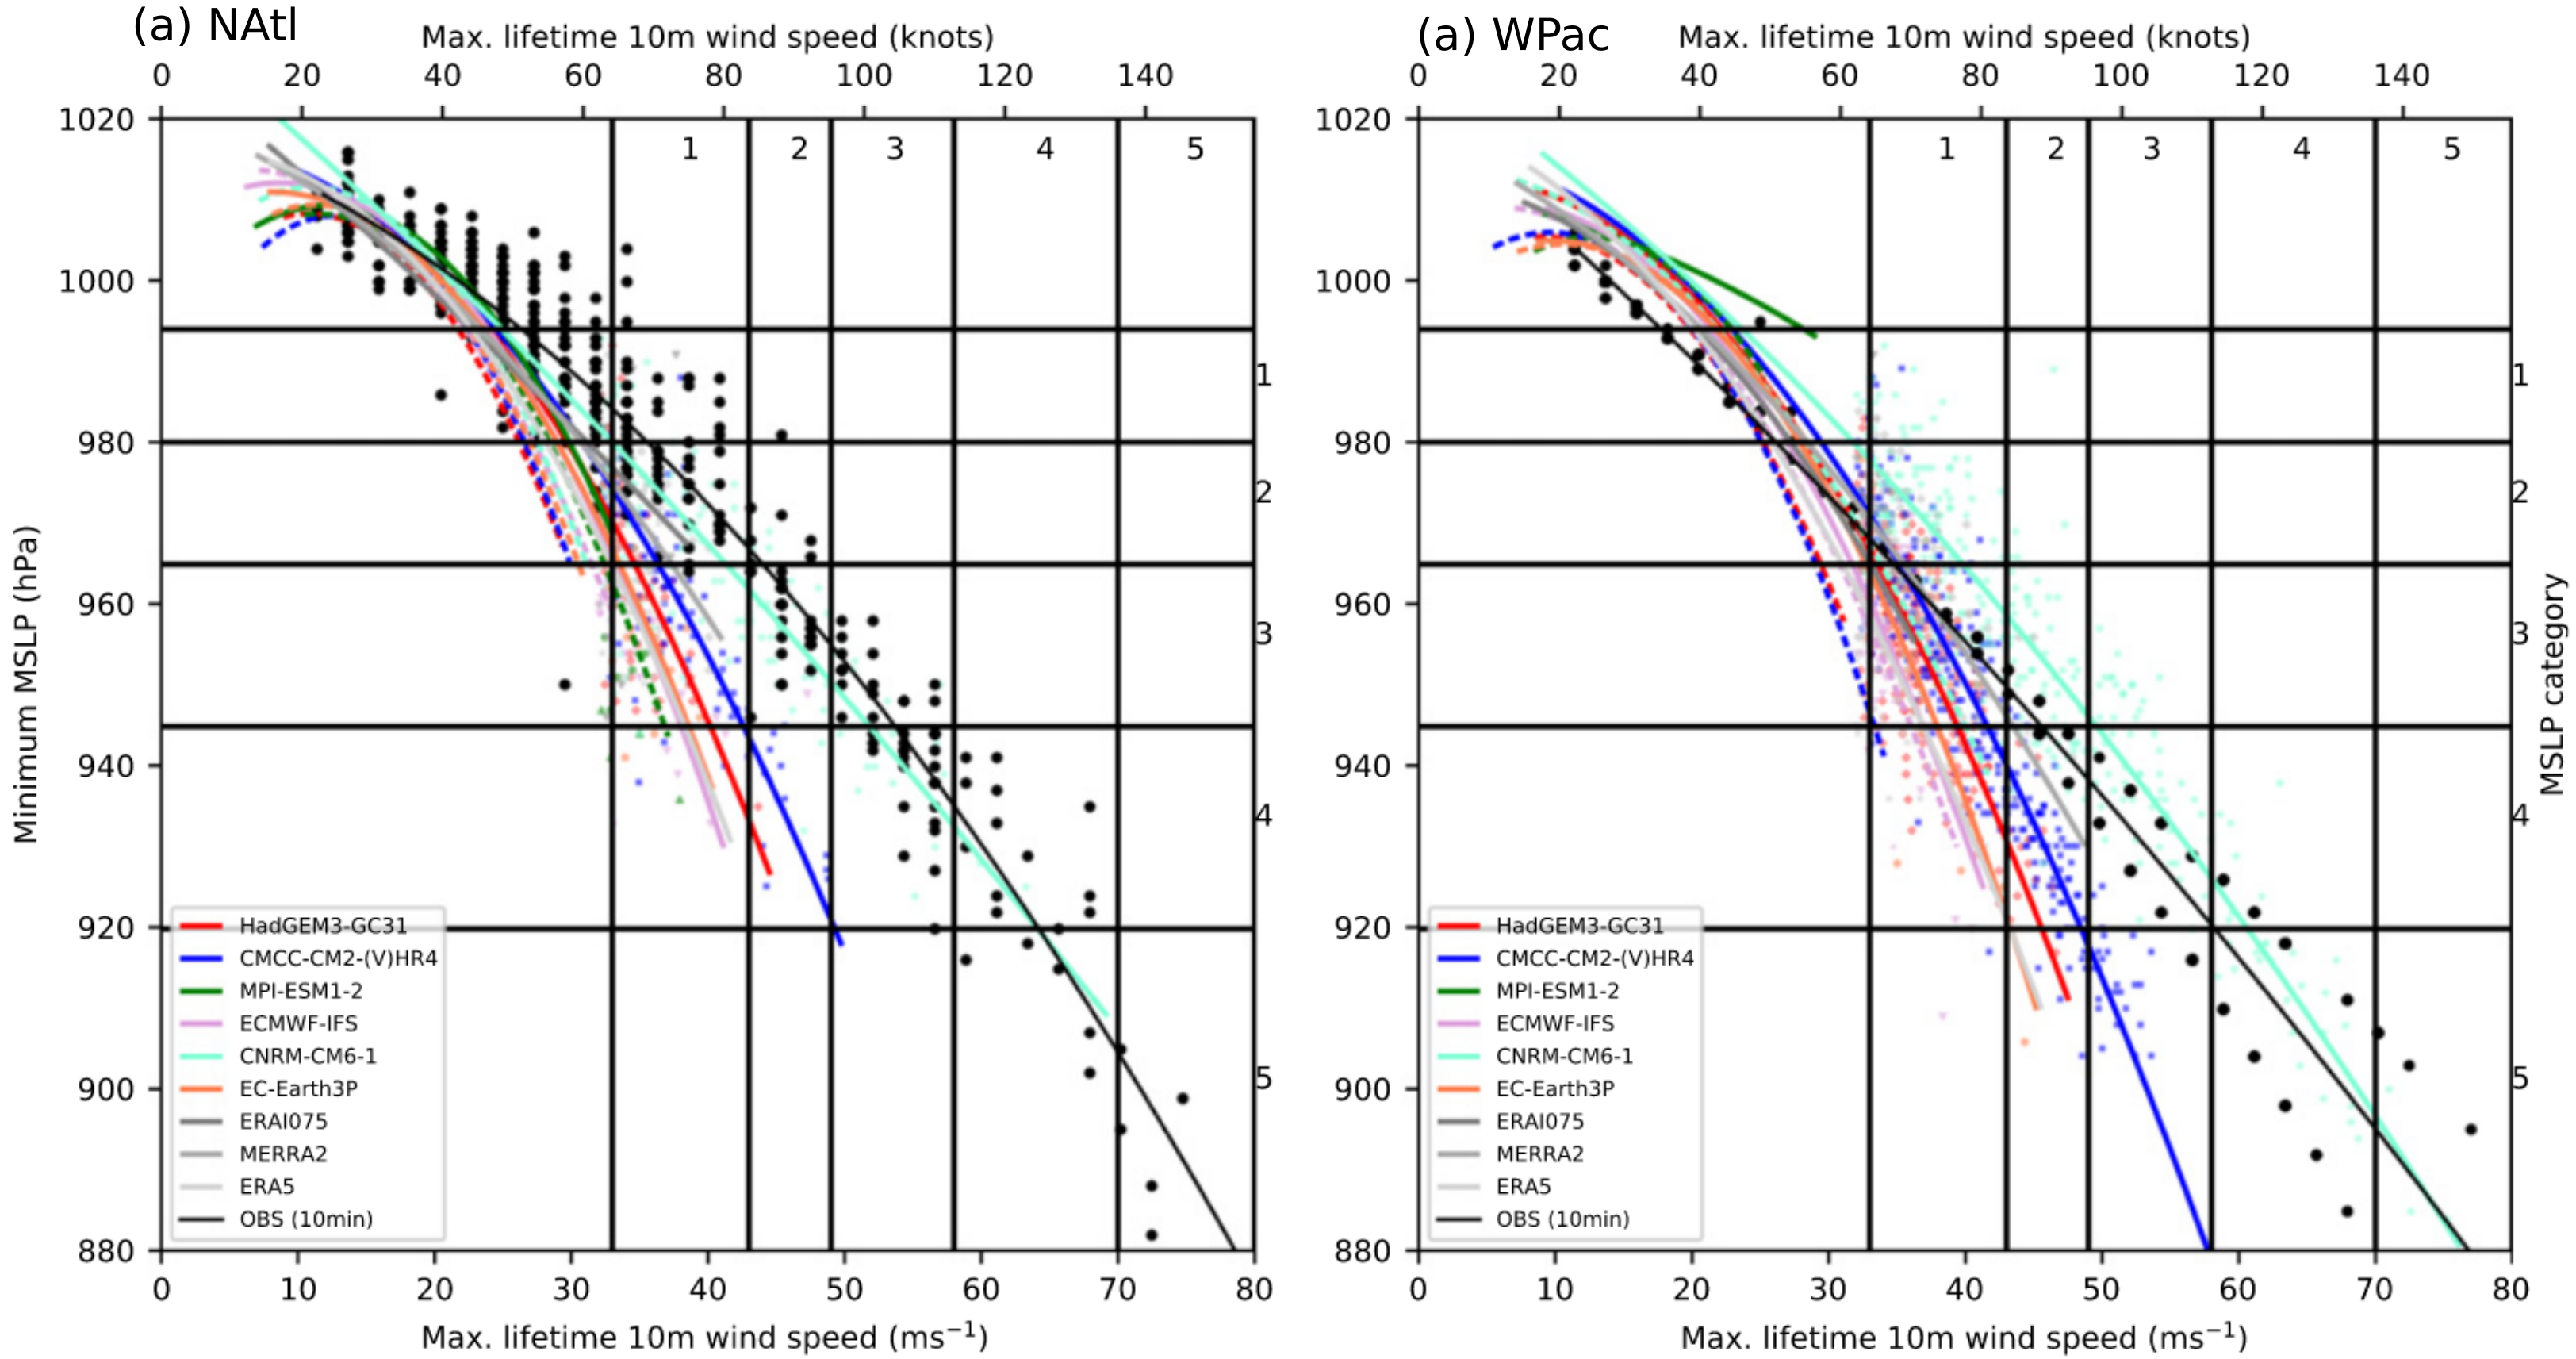
\includegraphics[width=\textwidth]{roberts_impact_2020_PV_NA_WP.png}
    \caption{Diagramme de relations vent~--~pression entre le vent maximum à \m{10} et le minimum de pression moyenne au niveau de la mer (\textit{Mean
        Sea-Level Pressure}, MSLP) dans les bassins Nord Atlantique (a) et Ouest Pacfique (b), pour \num{6} paires de modèles basse / haute résolution dans des
        simulations HighResMIP du tiers \num{1} (Runs atmosphériques forcées), ainsi que pour \num{3} réanalyses (en teintes de gris) et dans les observations
        (en noir). Les lignes pointillées indiquent les régressions pour les modèles basses résolution, et les lignes pleines pour les modèles haute résolution.
        Figure issue de \hbox{\cite{roberts_impact_2020}}.}
    \label{fig:roberts_PV_resolution}
\end{figure}

Les modèles ont depuis continué à s'améliorer, et s'ils souffrent toujours de la sous-estimation de l'intensité maximale, ils sont désormais capables de simuler
l'évolution du cycle de vie des TC, la répartition géographique, la saisonnalité des bassins d'activité ---~avec plus ou moins de succès selon les bassins, et
selon les modèles~---
\parencite{bengtsson_tropical_2007,zhao_simulations_2009,shaevitz_characteristics_2014}, ainsi que l'influence de l'Oscillation australe El Niño sur l'activité cyclonique
\parencite{vitart_simulation_1997,gualdi_changes_2008,camargo_experimental_2009}. La fréquence annuelle globale de HTV dans les GCM est toutefois très variable
selon les modèles, comme en atteste la \cref{fig:NTC_HighResMIP}. La résolution des modèles joue un rôle crucial dans la représentation des TC, y compris dans
la fréquence. La \cref{fig:NTC_HighResMIP} montre en effet que les modèles à plus haute résolution simulent généralement plus de HTV que ceux de résolution
inférieure \parencite{camargo_global_2013,roberts_impact_2020}. Cependant, elle montre aussi que la résolution ne peut expliquer à elle seule la sous-estimation
de la fréquence, puisque deux des paires de modèles sur la \cref{fig:NTC_HighResMIP} ne présentent qu'une amélioration marginale, voire pas d'amélioration dans
leur version haute résolution (EC-Earth3P, \cite{haarsma_highresmip_2020} et MPI-ESM1-2, \cite{gutjahr_max_2019}). La figure met aussi en évidence de fortes
différences de fréquence relatives à l'échelle des bassins géographiques. Le modèle CNRM-CM6-1 est par exemple le seul à surestimer l'activité dans le bassin
NAtl, aussi bien dans version basse que haute résolution\footnote{Dans CNRM-CM6-1, la surestimation de la fréquence relative dans le NAtl pour la version basse
    résolution semble due au couplage océan-atmosphère, car \cite{roberts_impact_2020,roberts_projected_2020} montre en effet que l'expérience réalisée avec des
SST prescrites produit une activité relative de \SI{11}{\percent}. En revanche pour les autres modèles, le couplage tend à réduire l'activité dans cette
région.} avec respectivement \SI{28}{\percent} et \SI{26}{\percent}, contre \SI{21}{\percent} dans les observations. La \cref{fig:roberts_PV_resolution}
présente les relations vent~--~pression (\textit{Wind-Pressure Relationship}, WPR) pour les modèles présentés dans la \cref{fig:NTC_HighResMIP}. Les diagrammes
vent~--~pression sont couramment utilisés comme diagnostique pour comparer la relation entre ces deux variables ---~reliées entre elles par l'équilibre du vent
gradient~--- avec celle issue des observations et mesurée pour la première fois par \cite{atkinson_tropical_1977}. Avec la \cref{fig:roberts_PV_resolution},
\cite{roberts_impact_2020} montre une intensification des HTV lors du passage à des résolutions supérieures, comprises entre \km{25} et \km{50}, sans pour
autant parvenir à reproduire la plage de valeur observée puisque la plupart des modèles peinent à dépasser la catégorie \num{2}~--~\num{3}. Ici encore, le
modèle CNRM-CM-6-1-HR constitue l'exception en simulant des TC particulièrement intenses, dépassant même les observations dans le bassin WPac. Dans le NAtl,
\cite{chauvin_future_2020} montre que l'intensité des HTV est encore accrue lorsque le modèle est utilisé dans sa configuration tournée-étirée pour atteindre
\km{15} de résolution (voir \cref{fig:rotated_streched}). Ce cas constitue une anomalie, d'autant plus que la version précédente du modèle utilisée dans les
simulations de \cite{daloz_impact_2012} ---~également en configuration tournée-étirée, à \km{50}~--- ne produit pas de HTV aussi intenses. Cette particularité
serait probablement liée aux différences de paramétrisation physiques entre les deux versions \parencite{chauvin_future_2020}, auquel cas il est possible que la
capacité du modèle ARPEGE à simuler des TC de catégorie \num{4} et \num{5} soit due à de mauvaises raisons. Il est néanmoins à noter que, bien qu'ils soient peu
nombreux, d'autres modèles à très haute résolution sont en mesure d'atteindre de tels niveaux d'intensité. C'est notamment le cas du modèle MRI-AGCM~3.2 avec
sa grille à \km{20} \parencite{murakami_future_2012}, le modèle HiFLOR du GFDL à \km{25} \parencite{murakami_simulation_2015} ainsi que CAM~5.1 dans sa
configuration à \km{25} \parencite{wehner_effect_2014}.

Depuis les premiers HTV simulés de \cite{manabe_tropical_1970}, les modèles se sont très nettement améliorés, autant par l'intermédiaire de l'augmentation de la
puissance de calcul permettant d'atteindre des résolutions de quelques dizaines de kilomètres à l'échelle globale, que par les paramétrisations physiques qui
les composent et le couplage avec diverses composantes, tous deux permettant de mieux décrire les processus inhérents aux cyclones tropicaux, et donc de mieux
les représenter dans les modèles. Si les modèles ne permettent toujours pas, pour la plupart, de reproduire pleinement l'amplitude de l'intensité observée, et
si les différences dans leur capacité à représenter les TC et leur activité sont encore grandes, ils n'ont néanmoins jamais été aussi aptes à
simuler l'activité cyclonique et sa variabilité de manière réaliste qu'aujourd'hui. Les modèles de climat constituent par conséquent le meilleur outil pour
tenter d'évaluer l'impact du réchauffement climatique sur l'activité cyclonique.

\subsection{Consensus actuel sur les projections futures}\label{sec:projections_futures}

\cite{christensen_climate_2013,knutson_tropical_2020,seneviratne_weather_2021}

\begin{figure}[tb]
    \centering
    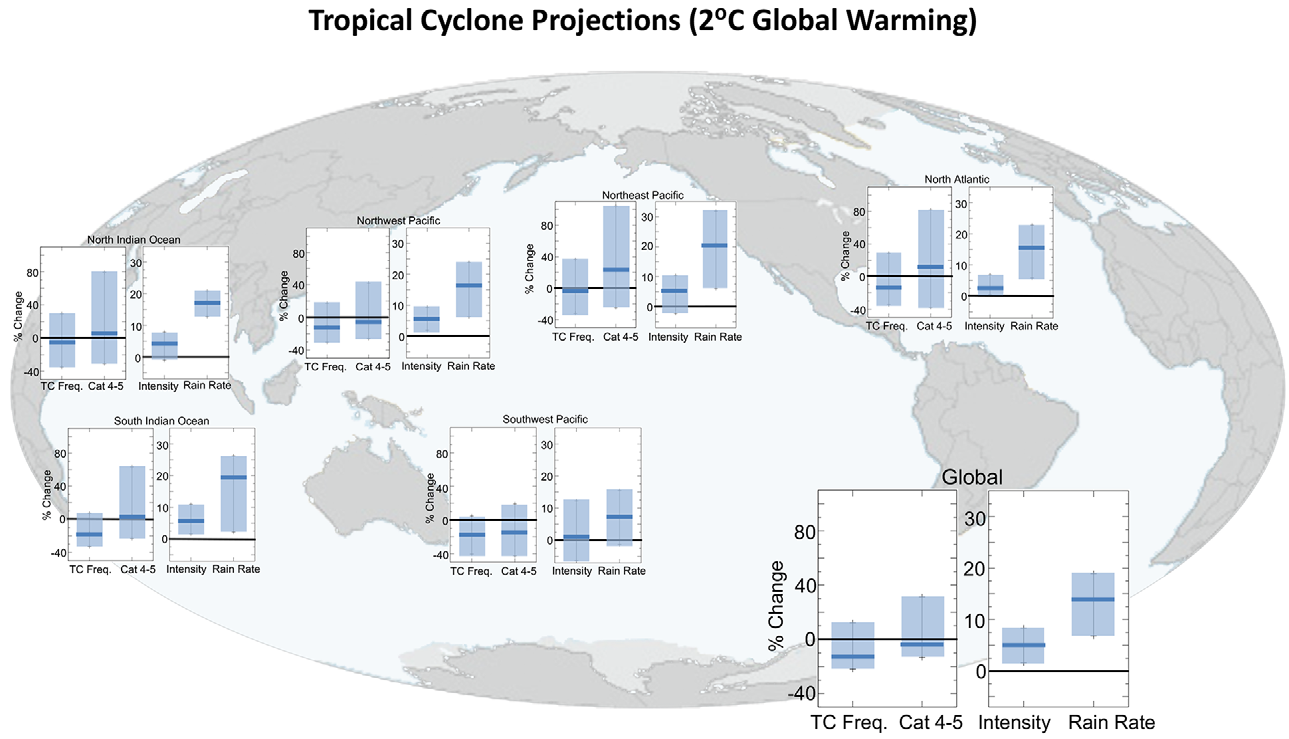
\includegraphics[width=\textwidth]{knutson_2020_projections.png}
    \caption{Résumé des projections simulées du changement de l'activité cyclonique par un réchauffement anthropique de l'atmosphère de \SI{2}{\degreeCelsius} à
        l'échelle globale par rapport à la climatologie \num{1986}~--~\num{2005}, pour les six bassins oćeaniques ainsi qu'à l'échelle du globe. Les changements
        sont exprimés pour la médiane (trait épais) avec son intervalle de confiance construit avec les pourcentiles \SI{5}{\percent}~--~\SI{95}{\percent} pour
        les deux métriques de fréquence, et \SI{10}{\percent}~--~\SI{90}{\percent} pour les métriques d'intensité et de précipitation. Figure issue de
        \cite{knutson_tropical_2020}.}
    \label{fig:projections_TC}
\end{figure}

\newpage
\subsection{Détection objective v.s indices de cyclogénèse}\label{sec:tracking_vs_indices}

\cite{horn_tracking_2014}

\begin{figure}[htbp]
    \centering
    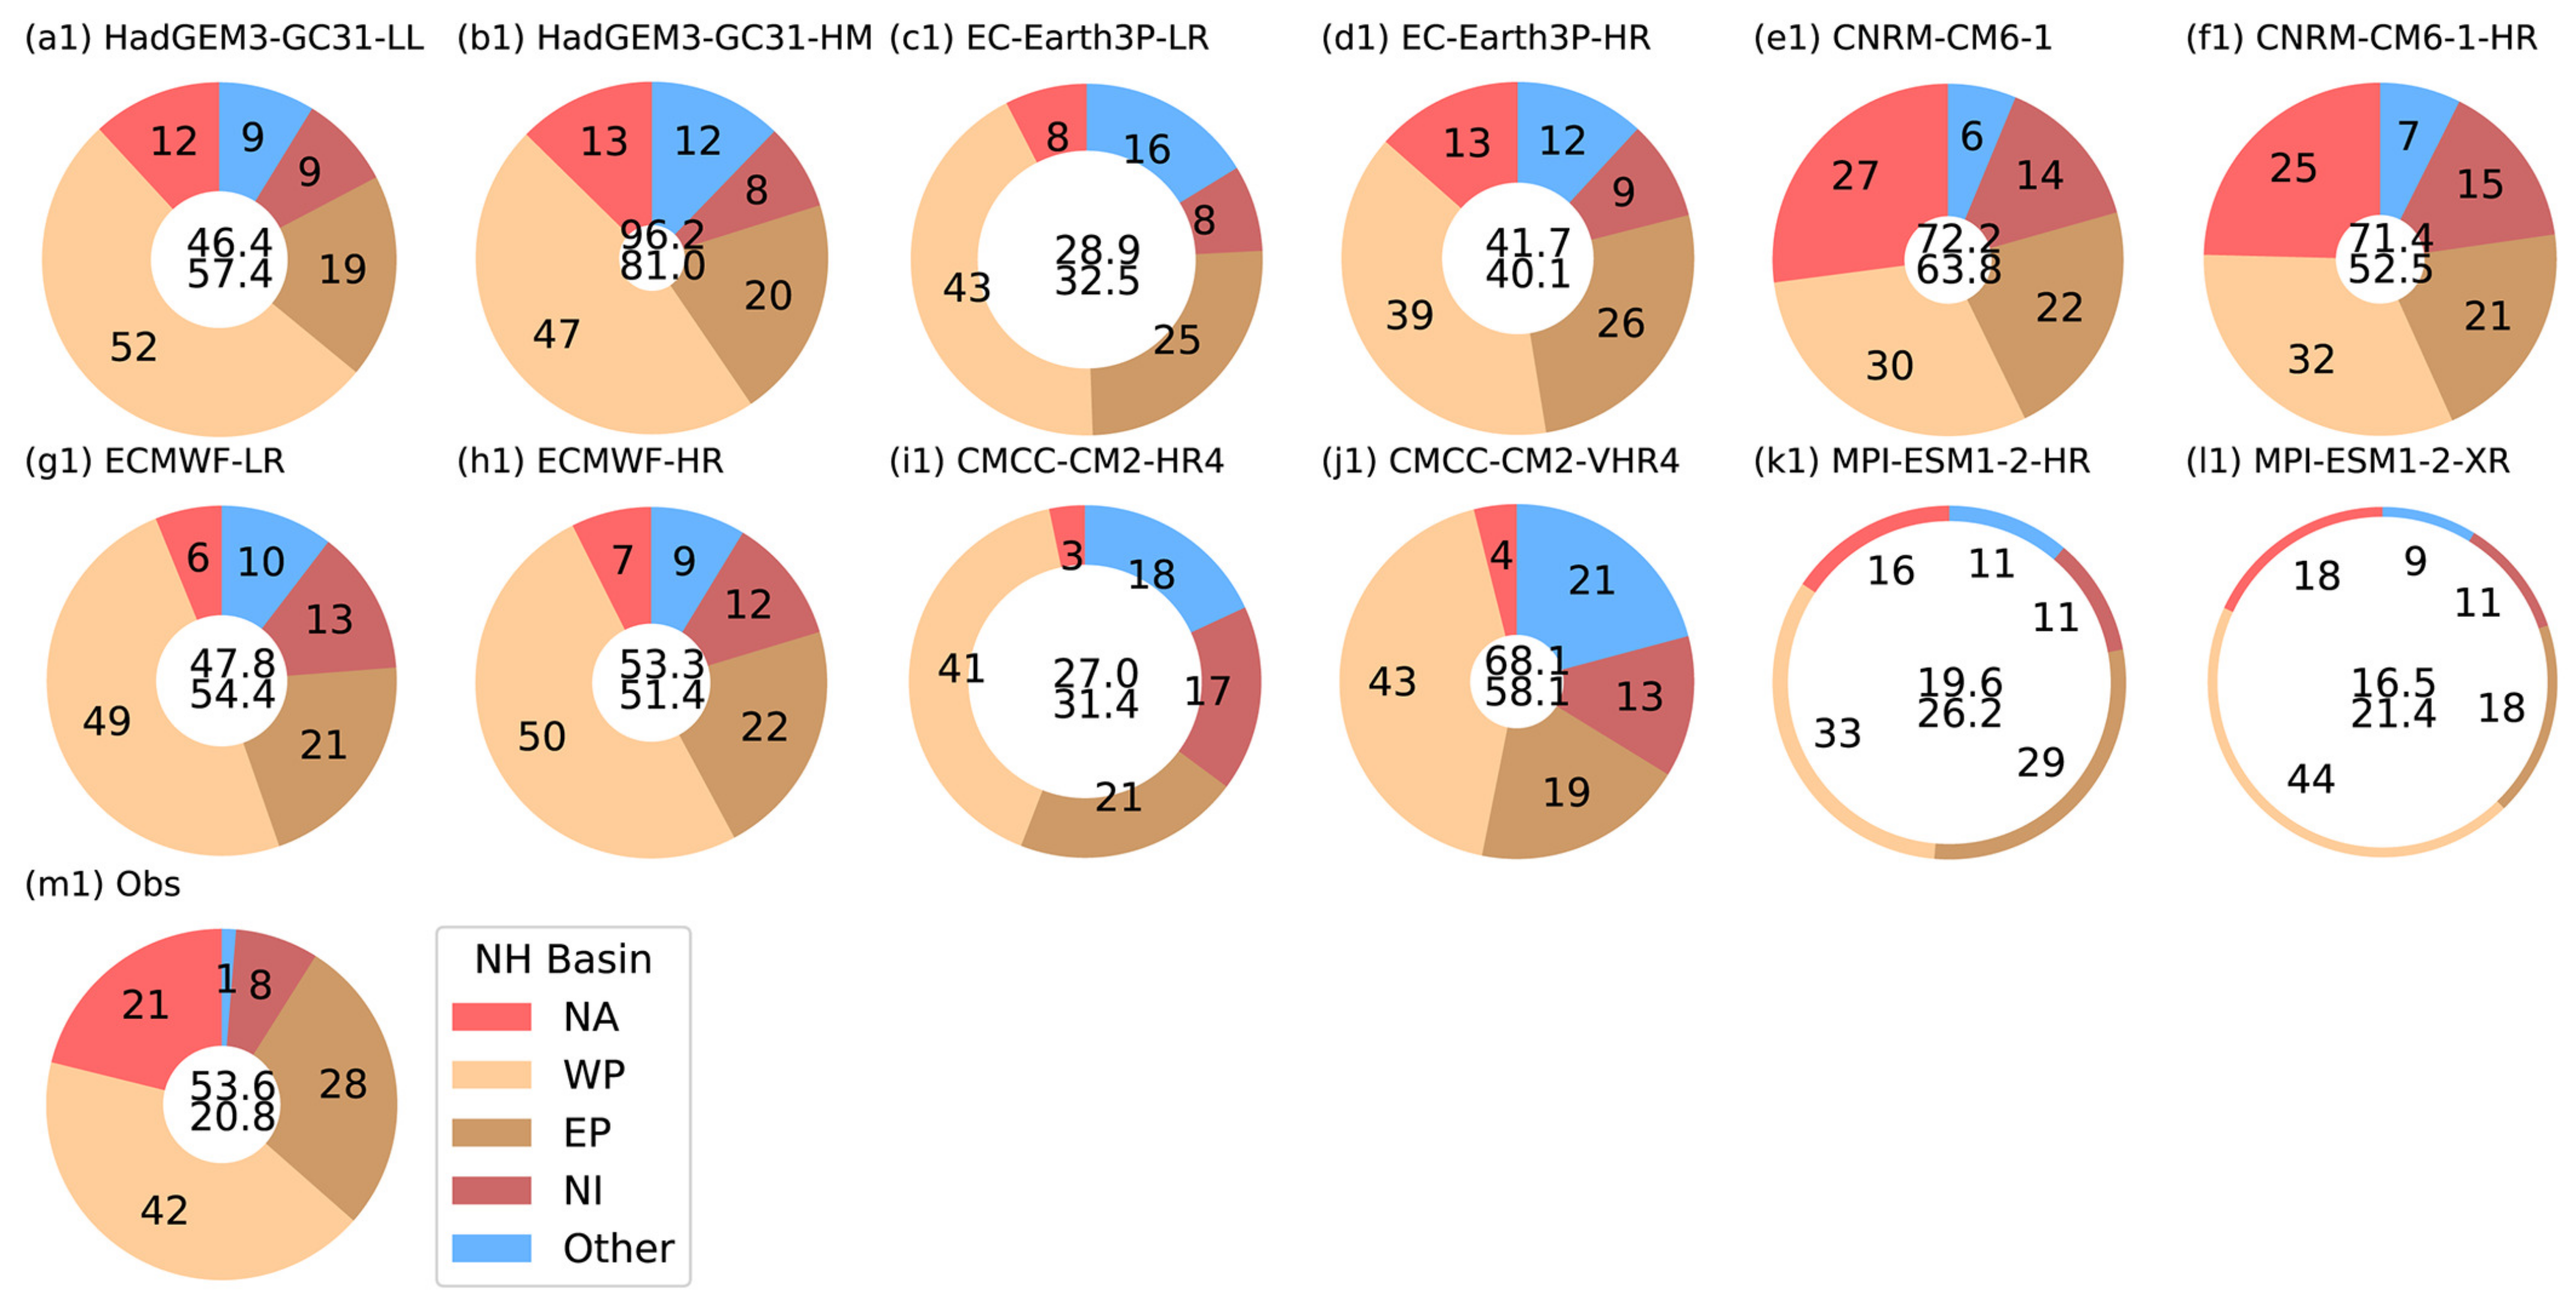
\includegraphics[width=\textwidth]{roberts_projected_2020_TRACKS_coupled.png}
    \caption{Comme pour la \cref{fig:NTC_HighResMIP}, mais où l'algorithme de détection TRACK \parencite{hodges_how_2017} est utilisé à la place de
    TempestExtreme \parencite{ullrich_tempestextremes_2017,zarzycki_assessing_2017}. Les réanalyses ne sont pas incluses. Figure issue de
    \cite{roberts_projected_2020}.}
    \label{fig:NTC_HighResMIP_TRACK}
\end{figure}

%----------------------------------------------------------------------------------------------------------------------
\section{Synthèse}

\end{document}
